\chapter{Superficies compactas}

\section{Superfies topológicas}

En primer lugar recordaremos algunos conceptos de Topología I para poder definir los nuevos conceptos de esta sección.

\begin{definicion}
    Diremos que un espacio topológico $X$ es T2 (o de \textbf{Haussforff}, o que satisface el \textbf{segundo axioma de separación}) si $\forall x,y \in X$ existe un abierto $U$ que contenga a $x$ y un abierto $V$ que contenga a $y$ tal que $U\cap V = \emptyset$.
        
        \begin{center}
            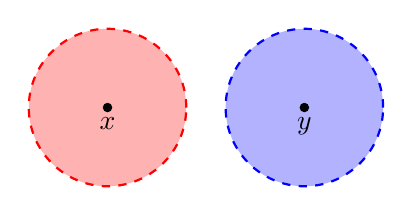
\begin{tikzpicture}
                \centering
    
                \def\radius{1}
    
                % Desactiva los caracteres conflictivos
                \shorthandoff{>} % Para poner puntas de flecha
    
                % Background
                \filldraw[thick, dashed, red, fill=red!30] (-1,0) circle (\radius);
                \filldraw[thick, dashed, blue, fill=blue!30] (1.5,0) circle (\radius);
    
                \filldraw (-1,0) circle (1.5pt) node[below] {$x$};
                \filldraw (1.5,0) circle (1.5pt) node[below] {$y$};
    
            \end{tikzpicture}
        \end{center}
\end{definicion}

\begin{definicion}
    Decimos que un espacio topológico $X$ es 2AN (o que cumple el \textbf{segundo axioma de numerabilidad}) si existe una base de la topología numerable.
\end{definicion}

Una vez recordados estos conceptos pasamos a las nuevas definiciones de esta sección:

\begin{definicion}
    Decimos que un espacio topológico $X$ es \textbf{localmente euclídeo} si para cada $x\in X$ existe un entorno abierto suyo que es homeomorfo a un abierto de $\bb{R}^n$.
\end{definicion}

\begin{definicion}
    Decimos que $S$ es una \textbf{superficie} si $S$ es un espacio topológico tal que $\forall x \in S$ existe un abierto que contiene a $x$ y que es homeomorfo a un abierto de $\bb{R}^2$. Además, pediremos que $S$ sea T2 (o Hausdorff) y 2AN (segundo axioma de numerabilidad).
\end{definicion}

\begin{ejemplo}\
    \begin{enumerate}
        \item $\bb{R}^2$ y $\bb{S}^2$ son superficies.
        \begin{proof}
            En el caso de $\bb{R}^2$ es trivial ya que para cualquier punto $x\in \bb{R}^2$ podemos considerar el total, $\bb{R}^2$ que es abierto, contiene a $x$ y es homeomorfo a sí mismo.\\

            En el caso de $\bb{S}^2$ podemos considerar para cada $x\in \bb{S}^2$ el conjunto $A = \bb{S}^2\setminus\{-x\}$, es decir, la esfera quitándole la antípoda. Sabemos que $A$ es abierto (ya que su complementario es $\{-x\}$ que es cerrado) y que contiene a $x$ (ya que $0\notin \bb{S}^2$). Además sabemos que $A$ es homeomorfo a $\bb{R}^2$ que es un abierto de $\bb{R}^2$ (el total).
        \end{proof}
        \item Cualquier abierto de una superficie es también una superficie. En particular, las bolas abiertas de $\bb{R}^2$ son también superficies.
        \begin{proof}
            Consideramos $A$ el abierto de la superficie $S$ y un punto cualquiera $x\in A$. Por ser $S$ una superficie existe un abierto $U$ que contiene a $x$ y que es homeomorfo (por $h$) a un abierto de $\bb{R}^2$. Consideramos entonces $A\cap U$ que es abierto por ser intersección de dos abiertos y que además contiene a $x$. Podemos considerar la restricción en el dominio del homeomorfismo $h$ a $A\cap U$ que seguirá siendo un homeomorfismo a un abierto de $\bb{R}^2$. Como esto se verifica para todo $x\in A$ tendremos que $A$ es una superficie.
        \end{proof}
        \item Sea $X=\{x\in \bb{R}^2 : \|x\|\leq r\} = \overline{B}(0,r)$. Entonces $X$ no es una superficie porque para los puntos $x$ con $\|x\| = r$ no existe un entorno abierto que lo contenga y que sea homeomorfo a un abierto de $\bb{R}^2$.
        \begin{proof}
            Tomamos un punto $x\in X$ con $\|x\|=r$. Si existiese $U$ entorno abierto suyo homeomorfo a un abierto $A$ de $\bb{R}^2$ entonces $\exists V$ entorno abierto de $x$ contenido en $U$ que es de la forma $V=B(x,r_0)\cap X$. Entonces $V$ es homeomorfo a un abierto $A'$ de $\bb{R}^2$ (ya que sería una restricción en el dominio del homeomorfismo entre $h:U\to A$). De esta forma tendríamos que como $V\setminus \{x\}$ es convexo debe ser simplemente conexo. Sin embargo, su imagen por homeomorfismo $h$ será $A'\setminus \{h(x)\}$ y como $h(x)$ está en el abierto $A'$ existe un radio $r_0'>0$ tal que $\overline{B}(h(x),r_0') \subseteq A'$. Pero el lazo dado por la frontera de dicha bola, $Fr(\overline{B}(h(x)r_0'))$ no es homotópicamente constante en $\bb{R}^2\setminus \{h(x)\}$. Por tanto este lazo no es homotópicamente constante en $A'\setminus\{h(x)\}$ por lo que $A'\setminus\{h(x)\}$ no es simplemente conexo. Esto prueba que $\overline{B}(0,r)$ no es una superficie.
        \end{proof}

        \item $\bb{S}^1\times \bb{R}$ y $\bb{S}^1\times \bb{S}^1$ son ejemplos de superficies. Esto se debe a que su recubridor universal es $\bb{R}^2$ luego sus aplicaciones recubridoras nos dan homeomorfismos locales desde abiertos de $\bb{R}^2$ en abiertos regularmente recubiertos de $\bb{S}^1 \times \bb{R}$ o $\bb{S}^1\times \bb{S}^1$.
    \end{enumerate}
\end{ejemplo}

\begin{observacion}
    Si $X$ es un espacio topológico localmente euclídeo entonces cumple las propiedades locales de $\bb{R}^n$. Por ejemplo, tiene una base de entornos numerable (es 1AN) y es localmente simplemente conexo. En particular, $X$ ha de tener recubridor universal.
\end{observacion}

\begin{definicion}
    Sea $S$ una superficie\footnote{siempre se entiende que es una superficie topológica} y $D$ un abierto dentro de $S$. Decimos que $D$ es un \textbf{disco regular} en $S$ si existe un abierto $D'$ tal que $D\subsetneq D'$ y un homeomorfismo $h:D'\to \bb{D}=\{x\in \bb{R}^2 : \|x\|<1\}=B((0,0),1)$ tal que $h(D)=\bb{D}_r=\{x\in \bb{R}^2 : \|x\|<r\}=B((0,0),r)$ con $0<r<1$.
\end{definicion}

\begin{ejemplo}\
    \begin{enumerate}
        \item Consideramos en $\bb{S}^2$:
        \begin{gather*}
            D = \{(x,y,z)\in \bb{S}^2 : z<r\} \text{ con } -1<r<1
        \end{gather*}
        En efecto es un disco regular. 
        \begin{proof}
            Como $-1<r<1$ tenemos que existe un $\veps >0$ tal que $r + \veps < 1$. Podemos fijar dicho $\veps$ y consideramos el siguiente conjunto
            \begin{gather*}
                D' = \{(x,y,z)\in \bb{S}^2 : z<r+\veps = r'\} \text{ con } -1<r'<1
            \end{gather*}
            En efecto tendremos que para cualquier punto $(x,y,z)\in D$ se tiene que $z<r<r'$ luego $(x,y,z)\in D'$. Además podemos considerar un punto $(x,y,z)\in \bb{S}^2$ tal que $z=r$ y tendremos que dicho punto está en $D'\setminus D$. Podemos concluir que $D\subsetneq D'$.

            \begin{figure}[H]
                \centering
                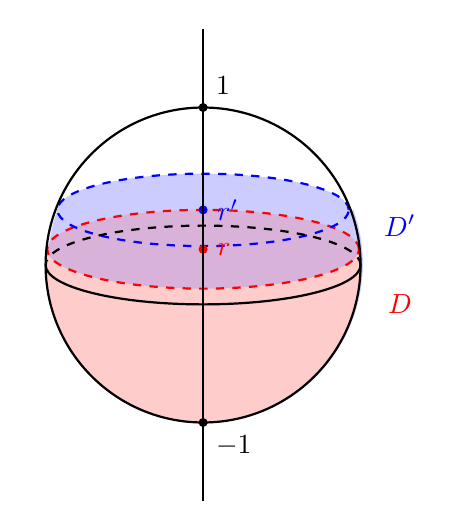
\begin{tikzpicture}
                    \shorthandoff{>}
                    \begin{scope}
                        % D y D'
                        \fill[blue!20] (-1.85, 0.7) arc (-200:20:2 and 2);
                        \fill[blue!20] (0,0.7) ellipse (1.85 and 0.46);

                        \fill[red!20] (-2,0.2) arc (-186:6:2 and 2);

                        \filldraw[thick, draw=red, fill=red!50!blue!30, dashed] (0,0.2) ellipse (1.98 and 0.5);

                        \draw[thick, blue, dashed] (0,0.7) ellipse (1.85 and 0.46);

                        \node[blue] at (2.5,0.5) {$D'$};
                        \node[red] at (2.5,-0.5) {$D$};

                        % r y r'
                        \node[draw, circle, red, fill=red, inner sep=1pt, label={[red]right:$r$}] at (0,0.2) {};
                        \node[draw, circle, blue, fill=blue, inner sep=1pt, label={[blue]right:$r'$}] at (0,0.7) {};

                        % Ejes
                        \draw[thick] (0,-3) -- (0,3);
                        \node[draw, circle, fill=black, inner sep=1pt, label=above right:$1$] at (0,2) {};
                        \node[draw, circle, fill=black, inner sep=1pt, label=below right:$-1$] at (0,-2) {};

                        % Esfera
                        \draw[thick] (0,0) circle [radius=2];
                        \draw[thick, dashed] (2,0) arc (0:180:2 and 0.5);
                        \draw[thick] (2,0) arc (0:-180:2 and 0.5);
                    \end{scope}
                \end{tikzpicture}
            \end{figure}
            
            Buscamos ahora un homeomorfismo $h:D'\to \bb{D}$ tal que $h(D)=\bb{D}_s$ con $0<s<1$. Pensamos en la proyección estereográfica desde el polo norte, $h:D'\to \bb{\bb{R}}^2$. Gráficamente lo podemos ver de la siguiente forma:

            \begin{figure}[H]
                \centering
                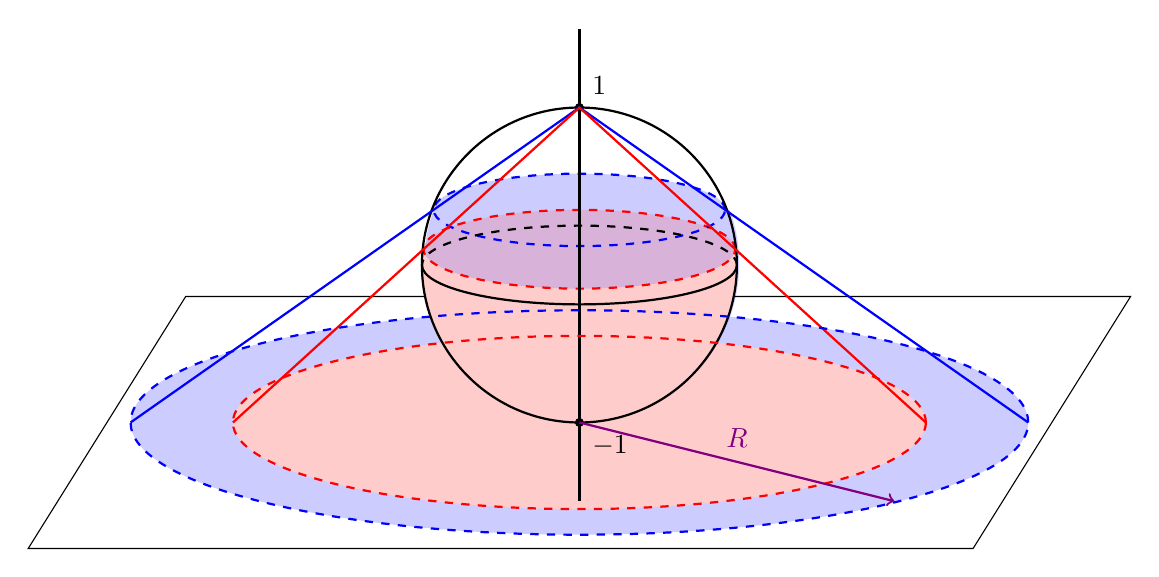
\begin{tikzpicture}
                    \shorthandoff{>}
                    \begin{scope}

                        \fill[thick, blue!20, dashed] (0,-2) ellipse (5.7 and 1.425);
                        \fill[thick, red!20, dashed] (0,-2) ellipse (4.4 and 1.1);

                        % D y D'
                        \fill[blue, opacity=0.2] (-1.85, 0.7) arc (-200:20:2 and 2);
                        \fill[blue!20] (0,0.7) ellipse (1.85 and 0.46);

                        \fill[red!20] (-2,0.2) arc (-186:6:2 and 2);

                        \filldraw[thick, draw=red, fill=red!50!blue!30, dashed] (0,0.2) ellipse (1.98 and 0.5);

                        \draw[thick, blue, dashed] (0,0.7) ellipse (1.85 and 0.46);

                        % Ejes
                        \draw[thick] (0,-3) -- (0,3);
                        \node[draw, circle, fill=black, inner sep=1pt, label=above right:$1$] at (0,2) {};
                        \node[draw, circle, fill=black, inner sep=1pt, label=below right:$-1$] at (0,-2) {};

                        % Esfera
                        \draw[thick] (0,0) circle [radius=2];
                        \draw[thick, dashed] (2,0) arc (0:180:2 and 0.5);
                        \draw[thick] (2,0) arc (0:-180:2 and 0.5);

                        % Plano suelo 
                        \draw (-1.95,-0.4) -- (-5, -0.4) -- (-7,-3.6) -- (5,-3.6) -- (7, -0.4) -- (1.95,-0.4);

                        \draw[thick, blue] (5.7 , -2) -- (0,2) -- (-5.7 , -2);
                        \draw[thick, red] (4.4 , -2) -- (0,2) -- (-4.4 , -2);
                        
                        \draw[thick, red, dashed] (0,-2) ellipse (4.4 and 1.1);
                        \draw[thick, blue, dashed] (0,-2) ellipse (5.7 and 1.425);

                        % Radio
                        \draw[thick, violet, ->] (0,-2) -- (4,-3);
                        \node[violet] at (2,-2.2) {$R$};
                    \end{scope}
                \end{tikzpicture}
            \end{figure}
        \end{proof}

        y llegamos a que existe un radio $R>0$ tal que podemos definir una nueva aplicación
        \Func{h'}{D'}{\bb{D}}{(x,y,z)}{\frac{1}{R}h(x,y,z)}
        que será un homeomorfismo (por serlo $h$). Además, es fácil ver que $h'(D) = \bb{D}_s$ con $0<s<1$.

        \item Consideramos la esfera sin el polo norte $D = \bb{S}^2\setminus \{(0,0,1)\}$ en $\bb{S}^2$. En este caso tendremos que no es un disco regular ya que el único abierto $D'$ que contiene estrictamente a $D$ es el total $D'=\bb{S}^2$ que sabemos que no es homeomorfo a ningún subconjunto de $\bb{R}^2$.

        \item $\bb{D}_r = B((0,0), r)\subseteq \bb{R}^2$ es un disco regular en $\bb{R}^2$ para todo $r\in \bb{R}^+$. Sin embargo, $\bb{D}_r$ no es regular en $S=\bb{D}_r$.
        
        \item En $\bb{R}^2$ consideramos el siguiente conjunto
        \begin{gather*}
            D=\bb{R}^2 \setminus \{(x,0) : x\geq 0\}
        \end{gather*}
        Entonces $D$ no puede ser un disco regular.
        \begin{proof}
            Si existiese un $D'$ que contiene a $D$ y contenido en $\bb{R}^2$ con $h: D' \to \bb{D}$ homeomorfismo tal que $h(D)= \bb{D}_r$ podemos tomar su restricción $h_{|D'\setminus D} : D'\setminus D  \to \bb{D}\setminus \bb{D}_r$ que seguirá siendo un homeomorfismo. Tenemos además que $D\subsetneq D \subseteq \bb{R}^2$ luego $D'\setminus D \subseteq \{(x,0) : x\geq 0\}$. Entonces tendremos que $(D'\setminus D)\setminus \{(x,0)\}$ no es convexo pero $h((D'\setminus D)\setminus \{(x,0)\}) = (\bb{D}\setminus \bb{D}_r)\setminus \{(h(x,0))\}$ es conexo por lo que no pueden ser homeomorfos y llegamos a contradicción.
        \end{proof}
    \end{enumerate}
\end{ejemplo}

\begin{lema}
    Sea $p_0$ un punto de una superficie $S$. Dado un entorno $U$ de $p_0$ existe $D$ disco regular que contiene a $p_0$ y está contenido en $U$. En particular, los discos regulares forman una base de la topología.
    \begin{proof}
        Como $S$ es una superficie, entonces para $p_0$ existe un abierto $V$ que contiene a $p_0$ y un homeomorfismo 
        \begin{gather*}
            \varphi : V \to \varphi(V)\subseteq \bb{R}^2
        \end{gather*}
        sobre $\varphi(V)$ que ha de ser abierto de $\bb{R}^2$. Ya que $\varphi(U\cap V)$ es un entorno de $\varphi(p_0)$ en $\bb{R}^2$ tenemos que existe un $R_0>0$ tal que
        \begin{gather*}
            B(\varphi(p_0), R_0)\subseteq \varphi(U\cap V)
        \end{gather*}
        Tomamos
        \begin{gather*}
            D=\varphi^{-1}\left(B\left(\varphi(p_0), \frac{R_0}{2}\right)\right)\\
            D'=\varphi^{-1}(B(\varphi(p_0), R_0))
        \end{gather*}
        Componiendo $\varphi$ con una transformación afín podemos llevar las bolas $B\left(\varphi(p_0), \frac{R_0}{2}\right)$ y $B(\varphi(p_0), R_0)$ a $\bb{D}_{\nicefrac{1}{2}}$ y $\bb{D}$ respectivamente.
    \end{proof}
\end{lema}

\begin{definicion}
    Sean $S_1$ y $S_2$ dos superficies conexas y disjuntas. Tomamos $D_1\subseteq S_1$ y $D_2\subseteq S_2$ discos regulares y consideramos un homeomorfismo $h: Fr(D_1)\to Fr(D_2)$. Sobre el espacio topológico $X=(S_1\setminus D_1)\cup (S_2\setminus D_2)$ consideramos la relación de equivalencia $R$ dada por
    \begin{gather*}
        x_1 R x_2 \sii \left\{
        \begin{array}{c}
            x_1=x_2\\
            \vee\\
            \{x_1,x_2\} = \{z, h(z)\} \text{ con } z\in Fr(D_1)
        \end{array}
        \right.
    \end{gather*}
    Denotamos por $S_1\# S_2$ al espacio topológico cociente de $X$ bajo la relación de equivalencia $R$ y lo llamaremos \textbf{suma conexa} de $S_1$ con $S_2$.
\end{definicion}

\begin{teo}
    El espacio topológico $S_1\#S_2$ es una superficie conexa que, salvo homeomorfismo, no depende de los discos $D_1$ y $D_2$ regulares ni del homeomorfismo $h$ entre sus fronteras.
\end{teo}

\begin{observacion}\
    \begin{enumerate}
        \item $S_1\#S_2 = S_2\#S_1$.

        \item Si $S_1$ es una superficie cualquiera y $S_2$ es la esfera $\bb{S}^2$, entonces 
        \begin{gather*}
            S_1\#S_2 = S_1\# \bb{S}^2 \cong S_1
        \end{gather*}
        % \begin{proof}
        %     Consideramos $D_1\subseteq S_1$ el disco regular de $S_1$ y $D_2\subseteq \bb{S}^2$ el disco regular de $\bb{S}^2$. Tenemos que $\bb{S}^2\setminus D_2$ es homeomorfo a un disco cerrado de $\bb{R}^2$. Pensamos ahora en el conjunto $\overline{D_1}$ que será homeomorfo a un disco cerrado de $\bb{S}^2$ y por tanto homeomorfo a $\bb{S}^2 \setminus D_2$. Si restringimos dicho homeomorfismo $h$ a la frontera tendremos que será un homeomorfismo $h_{|Fr(D_1)}:Fr(D_1) \to Fr(D_2)$ ya que $Fr(D_1) = Fr(\overline{D_1})$ y $Fr(D_2) = Fr(\bb{S}^2 \setminus D_2)$ y por tanto $S_1\#\bb{S}^2$ es homeomorfo a $S_1$ mediante $h$.
        % \end{proof}

        \item Si tenemos $n$ toros ($n\geq 2$) podemos definir 
        \begin{gather*}
            \bb{T}_n \equiv \text{suma conexa de los $n$ toros}
        \end{gather*}
        que recibe el nombre de \textbf{$n$-toro} o \textbf{esfera con $n$ asas}.

        \begin{figure}[H]
            \centering
            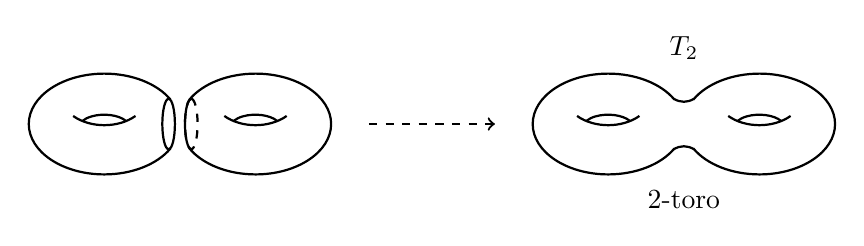
\begin{tikzpicture}[scale=0.8]
                \shorthandoff{>}
                \begin{scope}[scale=0.4, shift={(-10,0)}]
                    \begin{scope}[shift={(-3,0)}]
                        % Toro
                        % \draw[thick] (5,0) ellipse (3 and 2); % Exterior
                        \draw[thick] (-1.24,0.32) arc (225:315:1.75 and 1.25); % Agujero
                        \draw[thick] (0.86,0.12) arc (30:150:1 and 0.5);
                        % \draw[dashed] (5,0.2) ellipse (2.97 and 1.3); % Perímetro
                        \draw[thick] (-3,0) arc (-180:-29:3 and 2);
                        \draw[thick] (-3,0) arc (180:29:3 and 2);

                        % Boquete
                        \draw[thick] (2.55,0) ellipse (0.25 and 1); 
                    \end{scope}

                    \begin{scope}[shift={(3,0)}]
                        % Toro
                        % \draw[thick] (5,0) ellipse (3 and 2); % Exterior
                        \draw[thick] (-1.24,0.32) arc (225:315:1.75 and 1.25); % Agujero
                        \draw[thick] (0.86,0.12) arc (30:150:1 and 0.5);
                        % \draw[dashed] (5,0.2) ellipse (2.97 and 1.3); % Perímetro
                        \draw[thick] (3,0) arc (0:151:3 and 2);
                        \draw[thick] (3,0) arc (0:-151:3 and 2);

                        % Boquete
                        \draw[thick] (-2.55,1) arc (90:270:0.25 and 1);
                        \draw[thick, dashed] (-2.55,1) arc (90:-270:0.25 and 1);
                    \end{scope}
                \end{scope}

                \draw[thick, dashed, ->] (-1,0) -- (1,0);

                \begin{scope}[scale=0.4, shift={(10,0)}]
                    \begin{scope}[shift={(-3,0)}]
                        % Toro
                        % \draw[thick] (5,0) ellipse (3 and 2); % Exterior
                        \draw[thick] (-1.24,0.32) arc (225:315:1.75 and 1.25); % Agujero
                        \draw[thick] (0.86,0.12) arc (30:150:1 and 0.5);
                        % \draw[dashed] (5,0.2) ellipse (2.97 and 1.3); % Perímetro
                        \draw[thick] (-3,0) arc (-180:-29:3 and 2);
                        \draw[thick] (-3,0) arc (180:29:3 and 2); 
                    \end{scope}

                    \draw[thick, bend right=30] (-0.4,1) to (0.4,1);

                    \draw[thick, bend left=30] (-0.4,-1) to (0.4,-1);

                    \begin{scope}[shift={(3,0)}]
                        % Toro
                        % \draw[thick] (5,0) ellipse (3 and 2); % Exterior
                        \draw[thick] (-1.24,0.32) arc (225:315:1.75 and 1.25); % Agujero
                        \draw[thick] (0.86,0.12) arc (30:150:1 and 0.5);
                        % \draw[dashed] (5,0.2) ellipse (2.97 and 1.3); % Perímetro
                        \draw[thick] (3,0) arc (0:151:3 and 2);
                        \draw[thick] (3,0) arc (0:-151:3 and 2);

                    \end{scope}

                    \node at (0,3) {$\bb{T}_2$};
                    \node at (0, -3) {2-toro};
                \end{scope}
                
            \end{tikzpicture}
        \end{figure}
        \begin{figure}[H]
            \centering
            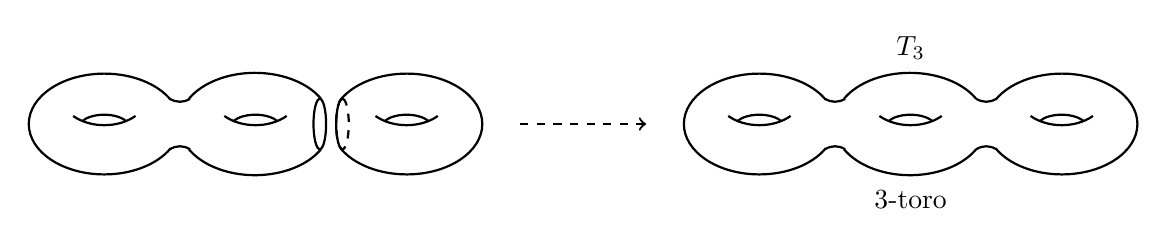
\begin{tikzpicture}[scale=0.8]
                \shorthandoff{>}
                \begin{scope}[scale=0.4, shift={(-16,0)}]
                    \begin{scope}[shift={(-3,0)}]
                        % Toro
                        % \draw[thick] (5,0) ellipse (3 and 2); % Exterior
                        \draw[thick] (-1.24,0.32) arc (225:315:1.75 and 1.25); % Agujero
                        \draw[thick] (0.86,0.12) arc (30:150:1 and 0.5);
                        % \draw[dashed] (5,0.2) ellipse (2.97 and 1.3); % Perímetro
                        \draw[thick] (-3,0) arc (-180:-29:3 and 2);
                        \draw[thick] (-3,0) arc (180:29:3 and 2); 
                    \end{scope}

                    \draw[thick, bend right=30] (-0.4,1) to (0.4,1);
                    \draw[thick, bend left=30] (-0.4,-1) to (0.4,-1);

                    \begin{scope}[shift={(3,0)}]
                        % Toro
                        \draw[thick] (-1.24,0.32) arc (225:315:1.75 and 1.25); % Agujero
                        \draw[thick] (0.86,0.12) arc (30:150:1 and 0.5);

                        % Exterior
                        \draw[thick] (2.6,1) arc (29:151:3 and 2);
                        \draw[thick] (2.6,-1) arc (-29:-151:3 and 2);

                        % Boquete
                        \draw[thick] (2.55,0) ellipse (0.25 and 1); 

                    \end{scope}

                    \begin{scope}[shift={(9,0)}]
                        % Toro
                        % \draw[thick] (5,0) ellipse (3 and 2); % Exterior
                        \draw[thick] (-1.24,0.32) arc (225:315:1.75 and 1.25); % Agujero
                        \draw[thick] (0.86,0.12) arc (30:150:1 and 0.5);
                        % \draw[dashed] (5,0.2) ellipse (2.97 and 1.3); % Perímetro
                        \draw[thick] (3,0) arc (0:151:3 and 2);
                        \draw[thick] (3,0) arc (0:-151:3 and 2);

                        % Boquete
                        \draw[thick] (-2.55,1) arc (90:270:0.25 and 1);
                        \draw[thick, dashed] (-2.55,1) arc (90:-270:0.25 and 1);

                    \end{scope}
                \end{scope}

                \draw[thick, dashed, ->] (-1,0) -- (1,0);

                \begin{scope}[scale=0.4, shift={(10,0)}]
                    \begin{scope}[shift={(-3,0)}]
                        % Toro
                        % \draw[thick] (5,0) ellipse (3 and 2); % Exterior
                        \draw[thick] (-1.24,0.32) arc (225:315:1.75 and 1.25); % Agujero
                        \draw[thick] (0.86,0.12) arc (30:150:1 and 0.5);
                        % \draw[dashed] (5,0.2) ellipse (2.97 and 1.3); % Perímetro
                        \draw[thick] (-3,0) arc (-180:-29:3 and 2);
                        \draw[thick] (-3,0) arc (180:29:3 and 2); 
                    \end{scope}

                    \draw[thick, bend right=30] (-0.4,1) to (0.4,1);
                    \draw[thick, bend left=30] (-0.4,-1) to (0.4,-1);

                    \begin{scope}[shift={(3,0)}]
                        % Toro
                        \draw[thick] (-1.24,0.32) arc (225:315:1.75 and 1.25); % Agujero
                        \draw[thick] (0.86,0.12) arc (30:150:1 and 0.5);

                        % Exterior
                        \draw[thick] (2.6,1) arc (29:151:3 and 2);
                        \draw[thick] (2.6,-1) arc (-29:-151:3 and 2);

                    \end{scope}

                    \node at (3,3) {$\bb{T}_3$};

                    \draw[thick, bend right=30] (5.6,1) to (6.4,1);
                    \draw[thick, bend left=30] (5.6,-1) to (6.4,-1);

                    \begin{scope}[shift={(9,0)}]
                        % Toro
                        % \draw[thick] (5,0) ellipse (3 and 2); % Exterior
                        \draw[thick] (-1.24,0.32) arc (225:315:1.75 and 1.25); % Agujero
                        \draw[thick] (0.86,0.12) arc (30:150:1 and 0.5);
                        % \draw[dashed] (5,0.2) ellipse (2.97 and 1.3); % Perímetro
                        \draw[thick] (3,0) arc (0:151:3 and 2);
                        \draw[thick] (3,0) arc (0:-151:3 and 2);
                    \end{scope}
                    \node at (3, -3) {3-toro};
                \end{scope}
                
            \end{tikzpicture}
        \end{figure}

        \item La suma conexa de $n$ planos proyectivos la llamaremos\footnote{no confundir con $\bb{R}\bb{P}^n$} \textbf{$n$ plano proyectivo}, $\bb{R}\bb{P}^2_n$.
    \end{enumerate}
\end{observacion}

\section{Presentaciones poligonales de superficies}

\begin{definicion}
    Consideramos el triángulo 
    \begin{gather*}
        T=\{(x,y)\in \bb{R}^2 : x\geq0,\ y\geq 0, x+y\leq 1\}
    \end{gather*}

    \begin{figure}[H]
        \centering
        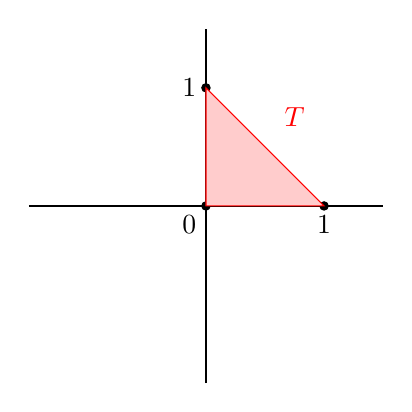
\begin{tikzpicture}[scale=1.5]
            \shorthandoff{>}
            % Ejes
            \draw[thick] (0,-1.5) -- (0,1.5);
            \draw[thick] (-1.5,0) -- (1.5,0);

            % Leyenda
            \filldraw (0,1) circle (1pt) node[left] {$1$};
            \filldraw (1,0) circle (1pt) node[below] {$1$};
            \filldraw (0,0) circle (1pt) node[below left] {$0$};
            \node[red] at (0.75,0.75) {$T$};

            \filldraw[draw=red, fill=red!20] (0,0) -- (1,0) -- (0,1) -- cycle;
        \end{tikzpicture}
    \end{figure}

    Decimos que un espacio topológico $X$ es un \textbf{triángulo} (topológico) si existe un homeomorfismo $h:T \to X$. En tal caso, llamaremos \textbf{vértices} de $X$ a la imagen mediante $h$ de los vértices de $T$ y \textbf{aristas} de $X$ a la imagen mediante $h$ de las aristas de $T$.
\end{definicion}

\begin{teo}[Teorema de Radó]
    Toda superficie compacta puede ser triangulada, es decir, la superficie puede verse como una unión finita triángulos (topológicos) de forma que dos triángulos distintos o bien son disjuntos o bien solo se intersecan en un vértice o solo en una arista.
\end{teo}

\begin{observacion}
    La idea de este teorema será que toda superficie compacta puede ser reconstruida pegando un número finito de triángulos a través de sus aristas.

    \begin{figure}[H]
        \centering
        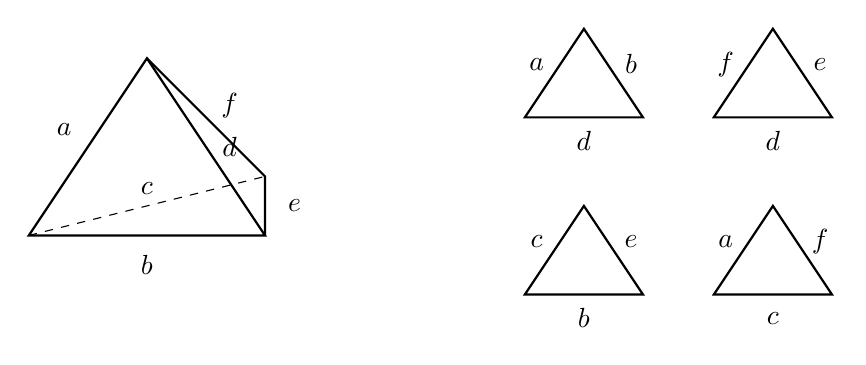
\begin{tikzpicture}[scale=1.5]
            \shorthandoff{>}
            \begin{scope}[shift={(0,0.5)}]
                % Pirámide
                \draw[thick] (0,0) -- (2,0) -- (1,1.5) -- cycle;
                \draw[thick] (2,0) -- (2,0.5) -- (1,1.5);
                \draw[dashed] (0,0) -- (2,0.5);

                % Leyenda
                \node at (0.3,0.9) {$a$};
                \node at (1,-0.25) {$b$};
                \node at (1,0.4) {$c$};
                \node at (1.7,0.75) {$d$};
                \node at (2.25,0.25) {$e$};
                \node at (1.7,1.1) {$f$};
            \end{scope}

            \begin{scope}[shift={(5,0)}]
                \begin{scope}[shift={(-0.8,1.5)}]
                    \draw[thick] (0,0) -- (1,0) -- (0.5,0.75) -- cycle;
                    % Leyenda
                    \node at (0.1,0.45) {$a$};
                    \node at (0.5,-0.2) {$d$};
                    \node at (0.9,0.45) {$b$};
                \end{scope}
                \begin{scope}[shift={(-0.8,0)}]
                    \draw[thick] (0,0) -- (1,0) -- (0.5,0.75) -- cycle;
                    % Leyenda
                    \node at (0.1,0.45) {$c$};
                    \node at (0.5,-0.2) {$b$};
                    \node at (0.9,0.45) {$e$};
                \end{scope}
                \begin{scope}[shift={(0.8,1.5)}]
                    \draw[thick] (0,0) -- (1,0) -- (0.5,0.75) -- cycle;
                    % Leyenda
                    \node at (0.1,0.45) {$f$};
                    \node at (0.5,-0.2) {$d$};
                    \node at (0.9,0.45) {$e$};
                \end{scope}
                \begin{scope}[shift={(0.8,0)}]
                    \draw[thick] (0,0) -- (1,0) -- (0.5,0.75) -- cycle;
                    % Leyenda
                    \node at (0.1,0.45) {$a$};
                    \node at (0.5,-0.2) {$c$};
                    \node at (0.9,0.45) {$f$};
                \end{scope}
            \end{scope}
        \end{tikzpicture}
    \end{figure}
\end{observacion}

\begin{definicion}
    Llamaremos presentación poligonal de una superficie compacta a una expresión de la forma 
    \begin{gather*}
        \cc{P} = \{a_1,...,a_n; w_1,...,w_m\} \text{ con } n,m\in \bb{N}
    \end{gather*}
    donde los $a_i$ son símbolos y los $w_j$ son expresiones del tipo
    \begin{gather*}
        w_i=a_{i1}^{\veps_{i1}}...a_{ik}^{\veps_{ik}}
    \end{gather*}
    donde $k\geq 3$ (es decir, hay al menos $3$ símbolos en la expresión $w_i$) y cada $\veps_{il}\in \{1,-1\}$ para cada $l\in\{1,...,k\}$. Y además, el número de veces que aparece cada símbolo en el total de los $w_i$ es $2$.
\end{definicion}

\begin{ejemplo}\
    \begin{enumerate}
        \item $\cc{P}=\{a,b;aba^{-1}b^{-1}\}$.
        \item $\cc{P}=\{a,b,c; aab, bcc^{-1}\}$.
        \item $\cc{P}=\{a,b,c,d; aab, bcd, cdd^{-1}\}$ no es una presentación ya que la $d$ aparece 3 veces.
    \end{enumerate}
\end{ejemplo}

\begin{definicion}
    A cada presentación poligonal $\cc{P}$ le asociaremos un espacio toloógico que denotaremos por $|\cc{P}|$ y que llamaremos la \textbf{realización geométrica de la presentación poligonal}. Su construcción es la siguiente
    \begin{enumerate}
        \item Para cada $w_i$ consideramos un polígono $P_i$ (regular) con número de lados igual al número de símbolos de $w_i$. Los $P_i$ serán disjuntos entre sí.
        \item Para cada $P_i$ asociado a un $w_i$ elegimos un lado cualquiera y en sentido contrario de las agujas del reloj, nombramos cada lado de $P_i$ con el nombre del símbolo. Además a cada lado le daremos la orientación contraria a las agujas del reloj si el exponente es $1$ y la orientación contraria si el exponente es $-1$.
        \item En el espacio topológico dado por la unión de todos los polígonos $P_i$ consideramos la relación la equivalencia que identifica los lados con igual nombre mediante el único homeomorfismo (aplicación que lleva un lado en otro sin cambiar el sentido de las flechas).
        \item Llamamos $|\cc{P}|$ al espacio cociente dado por la unión de los polígonos bajo la relación de equivalencia anterior.
    \end{enumerate}
\end{definicion}

\begin{ejemplo}
    $\cc{P}=\{a,b,c,d; abc^{-1}d, a^{-1}b^{-1}cd^{-1}\}$
    \begin{enumerate}
        \item \
        \begin{figure}[H]
            \centering
            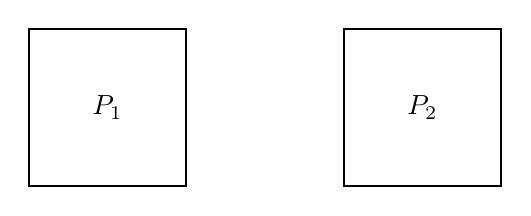
\begin{tikzpicture}
                \shorthandoff{>}
                \begin{scope}
                    \draw[thick] (-1,-1) -- (1,-1) -- (1,1) -- (-1,1) -- cycle;
                    \node at (0,0) {$P_1$};
                \end{scope}
                \begin{scope}[shift={(4,0)}]
                    \draw[thick] (-1,-1) -- (1,-1) -- (1,1) -- (-1,1) -- cycle;
                    \node at (0,0) {$P_2$};
                \end{scope}
            \end{tikzpicture}
        \end{figure}

        \item \
        \begin{figure}[H]
            \centering
            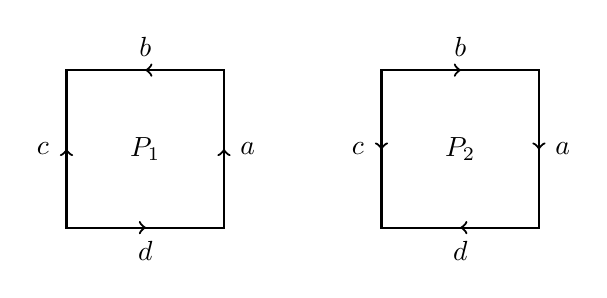
\begin{tikzpicture}
                \shorthandoff{>}
                \begin{scope}
                    \draw[thick] (-1,-1) -- (1,-1) -- (1,1) -- (-1,1) -- cycle;
                    \node at (0,0) {$P_1$};

                    % Aristas
                    \node at (1.3,0) {$a$};
                    \node at (0,1.3) {$b$};
                    \node at (-1.3,0) {$c$};
                    \node at (0,-1.3) {$d$};

                    %Sentidos
                    \draw[->, thick] (1,0) ++(0, -0.01) -- ++(0,0.01); %a
                    \draw[->, thick] (0,1) ++(0.01, 0) -- ++(-0.01,0); %b
                    \draw[->, thick] (-1,0) ++(0, -0.01) -- ++(0,0.01); %c
                    \draw[<-, thick] (0,-1) ++(0.01, 0) -- ++(-0.01,0); %d

                \end{scope}
                \begin{scope}[shift={(4,0)}]
                    \draw[thick] (-1,-1) -- (1,-1) -- (1,1) -- (-1,1) -- cycle;
                    \node at (0,0) {$P_2$};

                    % Aristas
                    \node at (1.3,0) {$a$};
                    \node at (0,1.3) {$b$};
                    \node at (-1.3,0) {$c$};
                    \node at (0,-1.3) {$d$};

                    %Sentidos
                    \draw[<-, thick] (1,0) ++(0, -0.01) -- ++(0,0.01); %a
                    \draw[<-, thick] (0,1) ++(0.01, 0) -- ++(-0.01,0); %b
                    \draw[<-, thick] (-1,0) ++(0, -0.01) -- ++(0,0.01); %c
                    \draw[->, thick] (0,-1) ++(0.01, 0) -- ++(-0.01,0); %d
                \end{scope}
            \end{tikzpicture}
        \end{figure}

        \item \
        \begin{figure}[H]
            \centering
            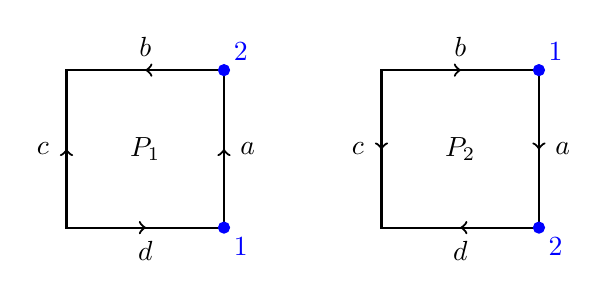
\begin{tikzpicture}
                \shorthandoff{>}
                \begin{scope}
                    \draw[thick] (-1,-1) -- (1,-1) -- (1,1) -- (-1,1) -- cycle;
                    \node at (0,0) {$P_1$};

                    % Aristas
                    \node at (1.3,0) {$a$};
                    \node at (0,1.3) {$b$};
                    \node at (-1.3,0) {$c$};
                    \node at (0,-1.3) {$d$};

                    %Sentidos
                    \draw[->, thick] (1,0) ++(0, -0.01) -- ++(0,0.01); %a
                    \draw[->, thick] (0,1) ++(0.01, 0) -- ++(-0.01,0); %b
                    \draw[->, thick] (-1,0) ++(0, -0.01) -- ++(0,0.01); %c
                    \draw[<-, thick] (0,-1) ++(0.01, 0) -- ++(-0.01,0); %d

                    %Identificaciones
                    \filldraw[blue] (1,1) circle (2pt) node[above right] {$2$};
                    \filldraw[blue] (1,-1) circle (2pt) node[below right] {$1$};
                \end{scope}
                \begin{scope}[shift={(4,0)}]
                    \draw[thick] (-1,-1) -- (1,-1) -- (1,1) -- (-1,1) -- cycle;
                    \node at (0,0) {$P_2$};

                    % Aristas
                    \node at (1.3,0) {$a$};
                    \node at (0,1.3) {$b$};
                    \node at (-1.3,0) {$c$};
                    \node at (0,-1.3) {$d$};

                    %Sentidos
                    \draw[<-, thick] (1,0) ++(0, -0.01) -- ++(0,0.01); %a
                    \draw[<-, thick] (0,1) ++(0.01, 0) -- ++(-0.01,0); %b
                    \draw[<-, thick] (-1,0) ++(0, -0.01) -- ++(0,0.01); %c
                    \draw[->, thick] (0,-1) ++(0.01, 0) -- ++(-0.01,0); %d

                    % Identificaciones 
                    \filldraw[blue] (1,1) circle (2pt) node[above right] {$1$};
                    \filldraw[blue] (1,-1) circle (2pt) node[below right] {$2$};
                \end{scope}
            \end{tikzpicture}
        \end{figure}
    \end{enumerate}
\end{ejemplo}

\begin{ejemplo}\
    \begin{figure}[H]
        \centering
        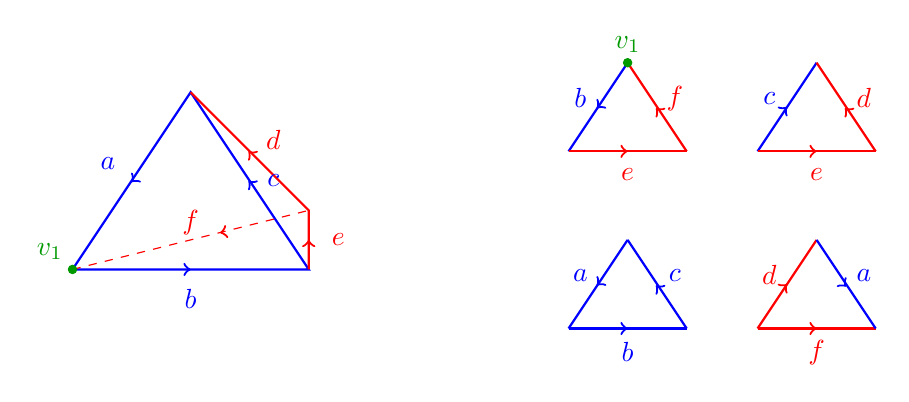
\begin{tikzpicture}[scale=1.5]
            \shorthandoff{>}
            \begin{scope}[shift={(0,0.5)}]
                % Pirámide
                \draw[thick, blue] (0,0) -- (2,0) -- (1,1.5) -- cycle;
                \draw[thick, red] (2,0) -- (2,0.5) -- (1,1.5);
                \draw[dashed, red] (0,0) -- (2,0.5);

                % Leyenda
                \node[blue] at (0.3,0.9) {$a$};
                \node[blue] at (1,-0.25) {$b$};
                \node[red] at (1,0.4) {$f$};
                \node[blue] at (1.7,0.75) {$c$};
                \node[red] at (2.25,0.25) {$e$};
                \node[red] at (1.7,1.1) {$d$};

                % Flechas
                \draw[<-, blue, thick] (0.5,0.75) ++(0, -0.01) -- ++(0.01,0.01); %a
                \draw[->, blue, thick] (1,0) ++(-0.01,0) -- ++(0.01,0); %b
                \draw[->, blue, thick] (1.5,0.75) ++(0, -0.01) -- ++(-0.01,0.01); %c
                \draw[->, red, thick] (1.5,1) ++(0, -0.01) -- ++(-0.01,0.01); %d
                \draw[->, red, thick] (2,0.25) ++(0, -0.01) -- ++(0,0.01); %e
                \draw[<-, red, thick] (1.25,0.32) ++(0, -0.01) -- ++(0.01,0.002); %f

                % Identificaciones
                \filldraw[green!60!black] (0,0) circle (1pt) node[above left] {$v_1$};
            \end{scope}

            \begin{scope}[shift={(5,0)}]
                \begin{scope}[shift={(-0.8,1.5)}]
                    % Triángulo
                    \draw[thick, blue] (0.5,0.75) -- (0,0); %1
                    \draw[thick, red] (0,0) -- (1,0); %2
                    \draw[thick, red] (1,0) -- (0.5,0.75); %3

                    % Leyenda
                    \node[blue] at (0.1,0.45) {$b$};
                    \node[red] at (0.5,-0.2) {$e$};
                    \node[red] at (0.9,0.45) {$f$};

                    % Flechas
                    \draw[->, blue, thick] (0.25,0.365) ++(0, 0.01) -- ++(-0.01,-0.01); %1
                    \draw[->, red, thick] (0.5,0) ++(-0.01,0) -- ++(0.01,0); %2
                    \draw[->, red, thick] (0.75,0.365) ++(0, -0.01) -- ++(-0.01,0.01); %3

                    % Identificación
                    \filldraw[green!60!black] (0.5,0.75) circle (1pt) node[above] {$v_1$};
                \end{scope}
                \begin{scope}[shift={(-0.8,0)}]
                    % Triángulo
                    \draw[thick, blue] (0.5,0.75) -- (0,0); %1
                    \draw[thick, blue] (0,0) -- (1,0); %2
                    \draw[thick, blue] (1,0) -- (0.5,0.75); %3

                    % Leyenda
                    \node[blue] at (0.1,0.45) {$a$};
                    \node[blue] at (0.5,-0.2) {$b$};
                    \node[blue] at (0.9,0.45) {$c$};

                    % Flechas
                    \draw[->, blue, thick] (0.25,0.365) ++(0, 0.01) -- ++(-0.01,-0.01); %1
                    \draw[->, blue, thick] (0.5,0) ++(-0.01,0) -- ++(0.01,0); %2
                    \draw[->, blue, thick] (0.75,0.365) ++(0, -0.01) -- ++(-0.01,0.01); %3
                \end{scope}
                \begin{scope}[shift={(0.8,1.5)}]
                    % Triángulo
                    \draw[thick, blue] (0.5,0.75) -- (0,0); %1
                    \draw[thick, red] (0,0) -- (1,0); %2
                    \draw[thick, red] (1,0) -- (0.5,0.75); %3

                    % Leyenda
                    \node[blue] at (0.1,0.45) {$c$};
                    \node[red] at (0.5,-0.2) {$e$};
                    \node[red] at (0.9,0.45) {$d$};

                    % Flechas
                    \draw[<-, blue, thick] (0.25,0.365) ++(0, 0.01) -- ++(-0.01,-0.01); %1
                    \draw[->, red, thick] (0.5,0) ++(-0.01,0) -- ++(0.01,0); %2
                    \draw[->, red, thick] (0.75,0.365) ++(0, -0.01) -- ++(-0.01,0.01); %3
                \end{scope}
                \begin{scope}[shift={(0.8,0)}]
                    % Triángulo
                    \draw[thick, red] (0.5,0.75) -- (0,0); %1
                    \draw[thick, red] (0,0) -- (1,0); %2
                    \draw[thick, blue] (1,0) -- (0.5,0.75); %3

                    % Leyenda
                    \node[red] at (0.1,0.45) {$d$};
                    \node[red] at (0.5,-0.2) {$f$};
                    \node[blue] at (0.9,0.45) {$a$};

                    % Flechas
                    \draw[<-, red, thick] (0.25,0.365) ++(0, 0.01) -- ++(-0.01,-0.01); %1
                    \draw[->, red, thick] (0.5,0) ++(-0.01,0) -- ++(0.01,0); %2
                    \draw[<-, blue, thick] (0.75,0.365) ++(0, -0.01) -- ++(-0.01,0.01); %3
                \end{scope}
            \end{scope}
        \end{tikzpicture}
    \end{figure}
    Tendríamos entonces $\cc{P}=\{a,b,c,d; abc, c^{-1}ed, a^{-1}d^{-1}f, bef\}$.
\end{ejemplo}

\begin{prop}
    El espacio topológico $|\cc{P}|$ asociado a una presentación poligonal $\cc{P}$ es una superficie compacta (posiblemente no conexa).
\end{prop}

\begin{observacion}
    Toda superficie compacta debe tener una presentación poligonal y recíprocamente, toda presentación poligonal nos da una superficie compacta. Como una misma superficie puede tener muchas (de hecho infinitas) presentaciones poligonales, nuestro objetivo será dada una presentación poligonal $\cc{P}$ llegar a otra presentación poligonal $\cc{P}'$ reconocible que represente a la misma superficie
\end{observacion}

\subsection{Transformaciones elementales}

Dada una presentación poligonal $\cc{P}$ vamos a ver una serie de transformaciones que, aunque cambian la presentación, no cambia la superficie asociada $|\cc{P}|$ (salvo homeomorfismo).

\subsubsection{Renombrar}
Dado un símbolo $a_{i_0}$ en $\cc{P}$ podemos cambiar su nombre por otro distinto $b_{i_0}$ que no esté siendo usado. También podemos cambiar el exponente de un símbolo las dos veces que aparezca este, es decir, cambiaríamos $a_i$ por $a_i^{-1}$ (en ambos lados a la vez).

\begin{figure}[H]
    \centering
    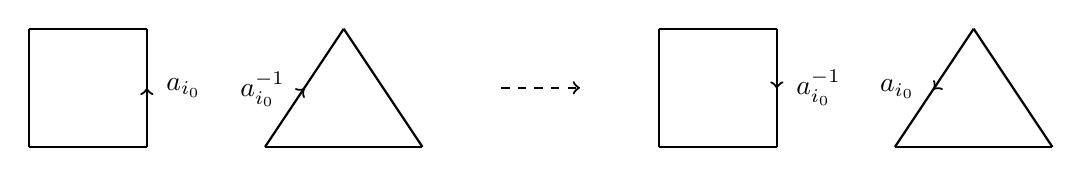
\begin{tikzpicture}
        \shorthandoff{>}
        \begin{scope}[shift={(-4,0)}]
            \begin{scope}[shift={(0,0)}]
                % Cuadrado
                \draw[thick] (0,1.5) -- (0,0); %1
                \draw[thick] (0,0) -- (1.5,0); %2
                \draw[thick] (1.5,0) -- (1.5,1.5); %3
                \draw[thick] (1.5,1.5) -- (0,1.5); %4

                % Leyenda
                % \node[label=left:{$a$}] at (0, 0.75) {}; %1
                % \node[label=below:{$b$}] at (0.75, 0) {}; %2
                \node[label=right:{$a_{i_0}$}] at (1.5, 0.75) {}; %3
                % \node[label=above:{$d$}] at (0.75, 1.5) {}; %4

                % Flechas
                % \draw[->, thick] (0,0.75) ++(0, 0.01) -- ++(0,-0.01); %1
                % \draw[->, thick] (0.75,0) ++(-0.01,0) -- ++(0.01,0); %2
                \draw[->, thick] (1.5,0.75) ++(0, -0.01) -- ++(0,0.01); %3
                % \draw[->, thick] (0.75,1.5) ++(0.01, -0.01) -- ++(-0.01,0); %4

            \end{scope}
            \begin{scope}[shift={(3,0)}]
                % Triángulo
                \draw[thick] (1,1.5) -- (0,0); %1
                \draw[thick] (0,0) -- (2,0); %2
                \draw[thick] (2,0) -- (1,1.5); %3

                % Leyenda
                \node[label=left:{$a_{i_0}^{-1}$}] at (0.5,0.73) {}; %1
                % \node[label=below:{$b$}] at (1, 0) {}; %2
                % \node[label=right:{$a_{i_0}$}] at (1.5, 0.73) {}; %3

                % Flechas
                \draw[<-, thick] (0.5,0.73) ++(0, 0.01) -- ++(-0.01,-0.01); %1
                % \draw[->, thick] (1,0) ++(-0.01,0) -- ++(0.01,0); %2
                % \draw[->, thick] (1.5,0.73) ++(0, -0.01) -- ++(-0.01,0.01); %3
            \end{scope}
        \end{scope}

        \draw[thick, dashed, ->] (2,0.75) -- (3,0.75);

        \begin{scope}[shift={(4,0)}]
            \begin{scope}[shift={(0,0)}]
                % Cuadrado
                \draw[thick] (0,1.5) -- (0,0); %1
                \draw[thick] (0,0) -- (1.5,0); %2
                \draw[thick] (1.5,0) -- (1.5,1.5); %3
                \draw[thick] (1.5,1.5) -- (0,1.5); %4

                % Leyenda
                % \node[label=left:{$a$}] at (0, 0.75) {}; %1
                % \node[label=below:{$b$}] at (0.75, 0) {}; %2
                \node[label=right:{$a_{i_0}^ {-1}$}] at (1.5, 0.75) {}; %3
                % \node[label=above:{$d$}] at (0.75, 1.5) {}; %4

                % Flechas
                % \draw[->, thick] (0,0.75) ++(0, 0.01) -- ++(0,-0.01); %1
                % \draw[->, thick] (0.75,0) ++(-0.01,0) -- ++(0.01,0); %2
                \draw[<-, thick] (1.5,0.75) ++(0, -0.01) -- ++(0,0.01); %3
                % \draw[->, thick] (0.75,1.5) ++(0.01, -0.01) -- ++(-0.01,0); %4

            \end{scope}
            \begin{scope}[shift={(3,0)}]
                % Triángulo
                \draw[thick] (1,1.5) -- (0,0); %1
                \draw[thick] (0,0) -- (2,0); %2
                \draw[thick] (2,0) -- (1,1.5); %3

                % Leyenda
                \node[label=left:{$a_{i_0}$}] at (0.5,0.73) {}; %1
                % \node[label=below:{$b$}] at (1, 0) {}; %2
                % \node[label=right:{$a_{i_0}$}] at (1.5, 0.73) {}; %3

                % Flechas
                \draw[->, thick] (0.5,0.73) ++(0, 0.01) -- ++(-0.01,-0.01); %1
                % \draw[->, thick] (1,0) ++(-0.01,0) -- ++(0.01,0); %2
                % \draw[->, thick] (1.5,0.73) ++(0, -0.01) -- ++(-0.01,0.01); %3
            \end{scope}
        \end{scope}
    \end{tikzpicture}
\end{figure}

\subsubsection{Subdividir}
Podemos cambiar un símbolo $a_{i_0}$ en $\cc{P}$ por dos símbolos $b_1b_2$ y $a_{i_0}^{-1}$ por $b_2^{-1}b_1^{-1}$, donde los símbolos $b_1$ y $b_2$ no están siendo usados.

\begin{figure}[H]
    \centering
    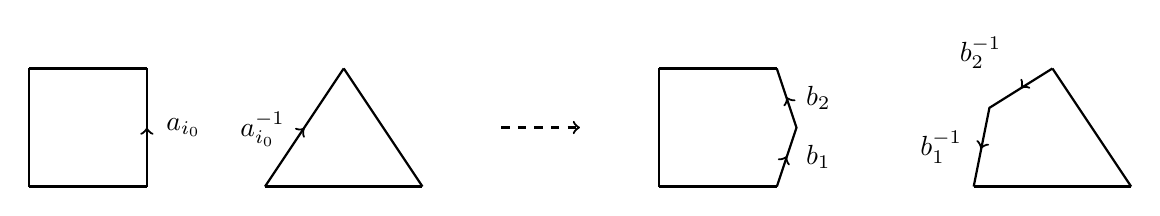
\begin{tikzpicture}
        \shorthandoff{>}
        \begin{scope}[shift={(-4,0)}]
            \begin{scope}[shift={(0,0)}]
                % Cuadrado
                \draw[thick] (0,1.5) -- (0,0); %1
                \draw[thick] (0,0) -- (1.5,0); %2
                \draw[thick] (1.5,0) -- (1.5,1.5); %3
                \draw[thick] (1.5,1.5) -- (0,1.5); %4

                % Leyenda
                % \node[label=left:{$a$}] at (0, 0.75) {}; %1
                % \node[label=below:{$b$}] at (0.75, 0) {}; %2
                \node[label=right:{$a_{i_0}$}] at (1.5, 0.75) {}; %3
                % \node[label=above:{$d$}] at (0.75, 1.5) {}; %4

                % Flechas
                % \draw[->, thick] (0,0.75) ++(0, 0.01) -- ++(0,-0.01); %1
                % \draw[->, thick] (0.75,0) ++(-0.01,0) -- ++(0.01,0); %2
                \draw[->, thick] (1.5,0.75) ++(0, -0.01) -- ++(0,0.01); %3
                % \draw[->, thick] (0.75,1.5) ++(0.01, -0.01) -- ++(-0.01,0); %4

            \end{scope}
            \begin{scope}[shift={(3,0)}]
                % Triángulo
                \draw[thick] (1,1.5) -- (0,0); %1
                \draw[thick] (0,0) -- (2,0); %2
                \draw[thick] (2,0) -- (1,1.5); %3

                % Leyenda
                \node[label=left:{$a_{i_0}^{-1}$}] at (0.5,0.73) {}; %1
                % \node[label=below:{$b$}] at (1, 0) {}; %2
                % \node[label=right:{$a_{i_0}$}] at (1.5, 0.73) {}; %3

                % Flechas
                \draw[<-, thick] (0.5,0.73) ++(0, 0.01) -- ++(-0.01,-0.01); %1
                % \draw[->, thick] (1,0) ++(-0.01,0) -- ++(0.01,0); %2
                % \draw[->, thick] (1.5,0.73) ++(0, -0.01) -- ++(-0.01,0.01); %3
            \end{scope}
        \end{scope}

        \draw[thick, dashed, ->] (2,0.75) -- (3,0.75);

        \begin{scope}[shift={(4,0)}]
            \begin{scope}[shift={(0,0)}]
                % Cuadrado
                \draw[thick] (0,1.5) -- (0,0); %1
                \draw[thick] (0,0) -- (1.5,0); %2
                \draw[thick] (1.5,0) -- (1.75,0.75) -- (1.5,1.5); %3
                \draw[thick] (1.5,1.5) -- (0,1.5); %4

                % Leyenda
                % \node[label=left:{$a$}] at (0, 0.75) {}; %1
                % \node[label=below:{$b$}] at (0.75, 0) {}; %2
                \node[label=right:{$b_1$}] at (1.625, 0.375) {}; %3
                \node[label=right:{$b_2$}] at (1.625, 1.125) {}; %3.5
                % \node[label=above:{$d$}] at (0.75, 1.5) {}; %4

                % Flechas
                % \draw[->, thick] (0,0.75) ++(0, 0.01) -- ++(0,-0.01); %1
                % \draw[->, thick] (0.75,0) ++(-0.01,0) -- ++(0.01,0); %2
                \draw[->, thick] (1.625, 0.375) ++(-0.01, -0.01) -- ++(0.01,0.02); %3
                \draw[->, thick] (1.625, 01.125) ++(0.01, -0.01) -- ++(-0.01,0.02); %3.5

                % \draw[->] (0.75,1.5) ++(0.01, -0.01) -- ++(-0.01,0); %4

            \end{scope}
            \begin{scope}[shift={(4,0)}]
                % Triángulo
                \draw[thick] (1,1.5) -- (0.2,1) -- (0,0); %1
                \draw[thick] (0,0) -- (2,0); %2
                \draw[thick] (2,0) -- (1,1.5); %3

                % Leyenda
                \node[label=above left:{$b_2^{-1}$}] at (0.6,1.25) {}; %1
                \node[label=left:{$b_1^{-1}$}] at (0.1,0.5) {}; %1.5
                % \node[label=below:{$b$}] at (1, 0) {}; %2
                % \node[label=right:{$a_{i_0}$}] at (1.5, 0.73) {}; %3

                % Flechas
                \draw[->, thick] (0.6,1.25) ++(0.01, 0.01) -- ++(-0.01,-0.01); %1
                \draw[->, thick] (0.1,0.5) ++(0, 0.01) -- ++(-0.01,-0.03); %1.5
                % \draw[->, thick] (1,0) ++(-0.01,0) -- ++(0.01,0); %2
                % \draw[->, thick] (1.5,0.73) ++(0, -0.01) -- ++(-0.01,0.01); %3
            \end{scope}
        \end{scope}
    \end{tikzpicture}
\end{figure}

\subsubsection{Consolidar}
Es el proceso contrario a subdividir. Si en las expresiones aparecen $a_{i_1}a_{i_2}$ y/o $a_{i_2}^{-1}a_{i_1}^{-1}$ dos veces (una de cada o dos de la misma), entones podemos cambiar $a_{i_1}a_{i_2}$ por $b_0$ y $a_{i_2}^{-1}a_{i_1}^{-1}$ por $b_0^{-1}$ (donde $b_0$ es un símbolo nuevo). Esto siempre se podrá hacer de forma que ninguna expresión se quede con menos de 3 símbolos.

\begin{figure}[H]
    \centering
    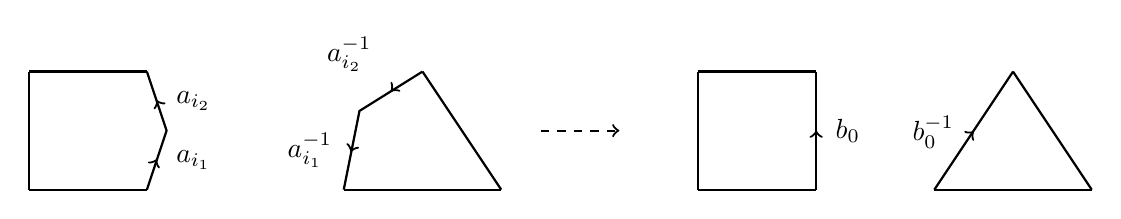
\begin{tikzpicture}
        \shorthandoff{>}
        \begin{scope}[shift={(-4.5,0)}]
            \begin{scope}[shift={(0,0)}]
                % Cuadrado
                \draw[thick] (0,1.5) -- (0,0); %1
                \draw[thick] (0,0) -- (1.5,0); %2
                \draw[thick] (1.5,0) -- (1.75,0.75) -- (1.5,1.5); %3
                \draw[thick] (1.5,1.5) -- (0,1.5); %4

                % Leyenda
                % \node[label=left:{$a$}] at (0, 0.75) {}; %1
                % \node[label=below:{$b$}] at (0.75, 0) {}; %2
                \node[label=right:{$a_{i_1}$}] at (1.625, 0.375) {}; %3
                \node[label=right:{$a_{i_2}$}] at (1.625, 1.125) {}; %3.5
                % \node[label=above:{$d$}] at (0.75, 1.5) {}; %4

                % Flechas
                % \draw[->, thick] (0,0.75) ++(0, 0.01) -- ++(0,-0.01); %1
                % \draw[->, thick] (0.75,0) ++(-0.01,0) -- ++(0.01,0); %2
                \draw[->, thick] (1.625, 0.375) ++(-0.01, -0.01) -- ++(0.01,0.02); %3
                \draw[->, thick] (1.625, 01.125) ++(0.01, -0.01) -- ++(-0.01,0.02); %3.5

                % \draw[->] (0.75,1.5) ++(0.01, -0.01) -- ++(-0.01,0); %4

            \end{scope}
            \begin{scope}[shift={(4,0)}]
                % Triángulo
                \draw[thick] (1,1.5) -- (0.2,1) -- (0,0); %1
                \draw[thick] (0,0) -- (2,0); %2
                \draw[thick] (2,0) -- (1,1.5); %3

                % Leyenda
                \node[label=above left:{$a_{i_2}^{-1}$}] at (0.6,1.25) {}; %1
                \node[label=left:{$a_{i_1}^{-1}$}] at (0.1,0.5) {}; %1.5
                % \node[label=below:{$b$}] at (1, 0) {}; %2
                % \node[label=right:{$a_{i_0}$}] at (1.5, 0.73) {}; %3

                % Flechas
                \draw[->, thick] (0.6,1.25) ++(0.01, 0.01) -- ++(-0.01,-0.01); %1
                \draw[->, thick] (0.1,0.5) ++(0, 0.01) -- ++(-0.01,-0.03); %1.5
                % \draw[->, thick] (1,0) ++(-0.01,0) -- ++(0.01,0); %2
                % \draw[->, thick] (1.5,0.73) ++(0, -0.01) -- ++(-0.01,0.01); %3
            \end{scope}
        \end{scope}

        \draw[thick, dashed, ->] (2,0.75) -- (3,0.75);

        \begin{scope}[shift={(4,0)}]
            \begin{scope}[shift={(0,0)}]
                % Cuadrado
                \draw[thick] (0,1.5) -- (0,0); %1
                \draw[thick] (0,0) -- (1.5,0); %2
                \draw[thick] (1.5,0) -- (1.5,1.5); %3
                \draw[thick] (1.5,1.5) -- (0,1.5); %4

                % Leyenda
                % \node[label=left:{$a$}] at (0, 0.75) {}; %1
                % \node[label=below:{$b$}] at (0.75, 0) {}; %2
                \node[label=right:{$b_0$}] at (1.5, 0.75) {}; %3
                % \node[label=above:{$d$}] at (0.75, 1.5) {}; %4

                % Flechas
                % \draw[->, thick] (0,0.75) ++(0, 0.01) -- ++(0,-0.01); %1
                % \draw[->, thick] (0.75,0) ++(-0.01,0) -- ++(0.01,0); %2
                \draw[->, thick] (1.5,0.75) ++(0, -0.01) -- ++(0,0.01); %3
                % \draw[->, thick] (0.75,1.5) ++(0.01, -0.01) -- ++(-0.01,0); %4

            \end{scope}
            \begin{scope}[shift={(3,0)}]
                % Triángulo
                \draw[thick] (1,1.5) -- (0,0); %1
                \draw[thick] (0,0) -- (2,0); %2
                \draw[thick] (2,0) -- (1,1.5); %3

                % Leyenda
                \node[label=left:{$b_0^{-1}$}] at (0.5,0.73) {}; %1
                % \node[label=below:{$b$}] at (1, 0) {}; %2
                % \node[label=right:{$a_{i_0}$}] at (1.5, 0.73) {}; %3

                % Flechas
                \draw[<-, thick] (0.5,0.73) ++(0, 0.01) -- ++(-0.01,-0.01); %1
                % \draw[->, thick] (1,0) ++(-0.01,0) -- ++(0.01,0); %2
                % \draw[->, thick] (1.5,0.73) ++(0, -0.01) -- ++(-0.01,0.01); %3
            \end{scope}
        \end{scope}
    \end{tikzpicture}
\end{figure}

\subsubsection{Reflejar}
Dada una expresión
\begin{gather*}
    w_i=a_{i_1}^{\veps_1}a_{i_2}^{\veps_2}...a_{i_l}^{\veps_l}
\end{gather*}
la podemos cambiar por
\begin{gather*}
    w_i' = a_{i_l}^{-\veps_l}...a_{i_2}^{-\veps_2}a_{i_1}^{-\veps_1}
\end{gather*}

\begin{figure}[H]
    \centering
    \begin{tikzpicture}
        \shorthandoff{>}
        \begin{scope}[shift={(-3.5,0)}]
            % Cuadrado
            \draw[thick] (0,1.5) -- (0,0); %1
            \draw[thick] (0,0) -- (1.5,0); %2
            \draw[thick] (1.5,0) -- (1.5,1.5); %3
            \draw[thick] (1.5,1.5) -- (0,1.5); %4

            \draw[dashed] (0.75,-0.1) -- (0.75,1.6);

            % Leyenda
            \node[label=left:{$c^{-1}$}] at (0, 0.75) {}; %1
            \node[label=below:{$d^{-1}$}] at (0.75, 0) {}; %2
            \node[label=right:{$a$}] at (1.5, 0.75) {}; %3
            \node[label=above:{$b$}] at (0.75, 1.5) {}; %4

            % Flechas
            \draw[<-, thick] (0,0.75) ++(0, 0.01) -- ++(0,-0.01); %1
            \draw[<-, thick] (0.75,0) ++(-0.01,0) -- ++(0.01,0); %2
            \draw[->, thick] (1.5,0.75) ++(0, -0.01) -- ++(0,0.01); %3
            \draw[->, thick] (0.75,1.5) ++(0.01, -0.01) -- ++(-0.01,0); %4

        \end{scope}

        \draw[thick, dashed, ->] (-0.5,0.75) -- (0.5,0.75);

        \begin{scope}[shift={(2,0)}]
            % Cuadrado
            \draw[thick] (0,1.5) -- (0,0); %1
            \draw[thick] (0,0) -- (1.5,0); %2
            \draw[thick] (1.5,0) -- (1.5,1.5); %3
            \draw[thick] (1.5,1.5) -- (0,1.5); %4

            % Leyenda
            \node[label=left:{$a^{-1}$}] at (0, 0.75) {}; %1
            \node[label=below:{$d$}] at (0.75, 0) {}; %2
            \node[label=right:{$c$}] at (1.5, 0.75) {}; %3
            \node[label=above:{$b^{-1}$}] at (0.75, 1.5) {}; %4

            % Flechas
            \draw[<-, thick] (0,0.75) ++(0, 0.01) -- ++(0,-0.01); %1
            \draw[->, thick] (0.75,0) ++(-0.01,0) -- ++(0.01,0); %2
            \draw[->, thick] (1.5,0.75) ++(0, -0.01) -- ++(0,0.01); %3
            \draw[<-, thick] (0.75,1.5) ++(0.01, -0.01) -- ++(-0.01,0); %4

        \end{scope}
    \end{tikzpicture}
\end{figure}

\subsubsection{Rotar}
Dada una expresión
\begin{gather*}
    w_i=a_{i_1}^{\veps_1}...a_{i_k}^{\veps_k}a_{i_{k+1}}^{\veps_{k+1}}...a_{i_l}^{\veps_l}
\end{gather*}
la podemos cambiar por
\begin{gather*}
    w_i'=a_{i_{k+1}}^{\veps_{k+1}}...a_{i_l}^{\veps_l}a_{i_1}^{\veps_1}...a_{i_k}^{\veps_k}
\end{gather*}

\begin{figure}[H]
    \centering
    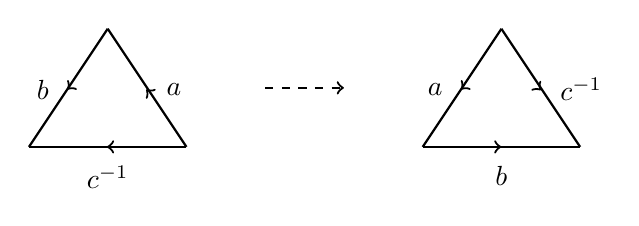
\begin{tikzpicture}
        \shorthandoff{>}

        \begin{scope}[shift={(-3.5,0)}]
            % Triángulo
            \draw[thick] (1,1.5) -- (0,0); %1
            \draw[thick] (0,0) -- (2,0); %2
            \draw[thick] (2,0) -- (1,1.5); %3

            % Leyenda
            \node[label=left:{$b$}] at (0.5,0.73) {}; %1
            \node[label=below:{$c^{-1}$}] at (1, 0) {}; %2
            \node[label=right:{$a$}] at (1.5, 0.73) {}; %3

            % Flechas
            \draw[->, thick] (0.5,0.73) ++(0, 0.01) -- ++(-0.01,-0.01); %1
            \draw[<-, thick] (1,0) ++(-0.01,0) -- ++(0.01,0); %2
            \draw[->, thick] (1.5,0.73) ++(0, -0.01) -- ++(-0.01,0.01); %3
        \end{scope}

        \draw[thick, dashed, ->] (-0.5,0.75) -- (0.5,0.75);

        \begin{scope}[shift={(1.5,0)}]
            % Triángulo
            \draw[thick] (1,1.5) -- (0,0); %1
            \draw[thick] (0,0) -- (2,0); %2
            \draw[thick] (2,0) -- (1,1.5); %3

            % Leyenda
            \node[label=left:{$a$}] at (0.5,0.73) {}; %1
            \node[label=below:{$b$}] at (1, 0) {}; %2
            \node[label=right:{$c^{-1}$}] at (1.5, 0.73) {}; %3

            % Flechas
            \draw[->, thick] (0.5,0.73) ++(0, 0.01) -- ++(-0.01,-0.01); %1
            \draw[->, thick] (1,0) ++(-0.01,0) -- ++(0.01,0); %2
            \draw[<-, thick] (1.5,0.73) ++(0, -0.01) -- ++(-0.01,0.01); %3
        \end{scope}
    \end{tikzpicture}
\end{figure}

\subsubsection{Cortar}
Dada una expresión
\begin{gather*}
    w_i=a_{i_1}^{\veps_1}...a_{i_k}^{\veps_k}a_{i_{k+1}}^{\veps_{k+1}}...a_{i_l}^{\veps_l}
\end{gather*}
podemos sustituirla por las dos expresiones
\begin{gather*}
    w_i' = a_{i_1}^{\veps_1}...a_{i_k}^{\veps_k}b\ \ ,\ \ w_i'' = b^{-1}a_{i_{k+1}}^{\veps_{k+1}}...a_{i_l}^{\veps_l}
\end{gather*}
Esto se podrá hacer siempre que $w_i'$ y $w_i''$ se queden con al menos de 3 símbolos.

\begin{figure}[H]
    \centering
    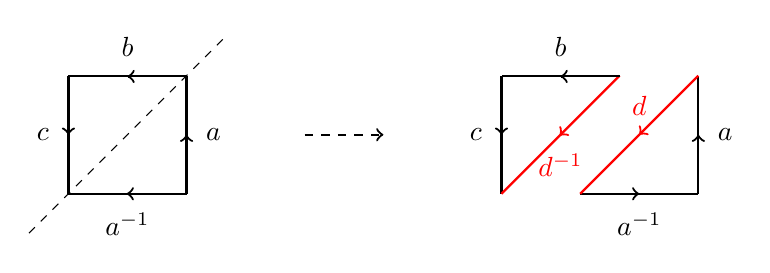
\begin{tikzpicture}
        \shorthandoff{>}
        \begin{scope}[shift={(-3.5,0)}]
            % Cuadrado
            \draw[thick] (0,1.5) -- (0,0); %1
            \draw[thick] (0,0) -- (1.5,0); %2
            \draw[thick] (1.5,0) -- (1.5,1.5); %3
            \draw[thick] (1.5,1.5) -- (0,1.5); %4

            \draw[dashed] (-0.5,-0.5) -- (2,2);

            % Leyenda
            \node[label=left:{$c$}] at (0, 0.75) {}; %1
            \node[label=below:{$a^{-1}$}] at (0.75, 0) {}; %2
            \node[label=right:{$a$}] at (1.5, 0.75) {}; %3
            \node[label=above:{$b$}] at (0.75, 1.5) {}; %4

            % Flechas
            \draw[->, thick] (0,0.75) ++(0, 0.01) -- ++(0,-0.01); %1
            \draw[<-, thick] (0.75,0) ++(-0.01,0) -- ++(0.01,0); %2
            \draw[->, thick] (1.5,0.75) ++(0, -0.01) -- ++(0,0.01); %3
            \draw[->, thick] (0.75,1.5) ++(0.01, -0.01) -- ++(-0.01,0); %4

        \end{scope}

        \draw[thick, dashed, ->] (-0.5,0.75) -- (0.5,0.75);

        \begin{scope}[shift={(2,0)}]
            % Cuadrado
            \draw[thick] (0,1.5) -- (0,0); %1
            \draw[thick, red] (0,0) -- (1.5,1.5); %2-3
            \draw[thick] (1.5,1.5) -- (0,1.5); %4

            % Leyenda
            \node[label=left:{$c$}] at (0, 0.75) {}; %1
            \node[label={[red]below:{$d^{-1}$}}] at (0.75, 0.75) {}; %2-3
            \node[label=above:{$b$}] at (0.75, 1.5) {}; %4

            % Flechas
            \draw[->, thick] (0,0.75) ++(0, 0.01) -- ++(0,-0.01); %1
            \draw[<-, thick, red] (0.75,0.75) ++(-0.01, -0.01) -- ++(0.01,0.01); %2-3
            \draw[->, thick] (0.75,1.5) ++(0.01, -0.01) -- ++(-0.01,0); %4

        \end{scope}

        \begin{scope}[shift={(3,0)}]
            % Cuadrado
            \draw[thick] (0,0) -- (1.5,0); %2
            \draw[thick] (1.5,0) -- (1.5,1.5); %3
            \draw[thick, red] (1.5,1.5) -- (0,0); %4-1

            % Leyenda
            \node[label=below:{$a^{-1}$}] at (0.75, 0) {}; %2
            \node[label=right:{$a$}] at (1.5, 0.75) {}; %3
            \node[label={[red]above:{$d$}}] at (0.75, 0.75) {}; %4-1

            % Flechas
            \draw[->, thick] (0.75,0) ++(-0.01,0) -- ++(0.01,0); %2
            \draw[->, thick] (1.5,0.75) ++(0, -0.01) -- ++(0,0.01); %3
            \draw[->, thick, red] (0.75,0.75) ++(0.01, 0.01) -- ++(-0.01,-0.01); %4-1

        \end{scope}
    \end{tikzpicture}
\end{figure}

\subsubsection{Pegar}
Es la operación opuesta a cortar. Dadas dos expresiones de la forma 
\begin{gather*}
    w_i' = a_{i_1}^{\veps_1}...a_{i_k}^{\veps_k}a_{i_0}\ \ ,\ \ w_i'' = a_{i_0}^{-1}a_{j_{1}}^{\veps_{1}}...a_{j_l}^{\veps_l}
\end{gather*}
las podemos sustituir por una única
\begin{gather*}
    w = a_{i_1}^{\veps_1}...a_{i_k}^{\veps_k}a_{j_{1}}^{\veps_{1}}...a_{j_l}^{\veps_l}
\end{gather*}

\begin{figure}[H]
    \centering
    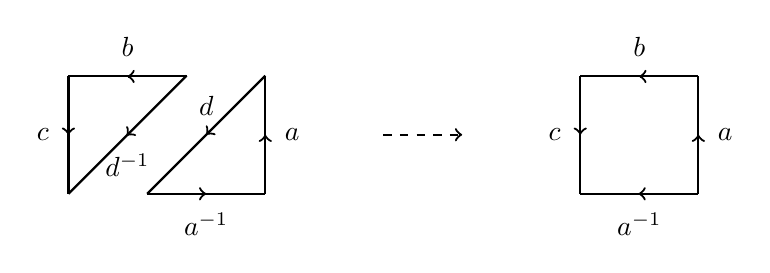
\begin{tikzpicture}
        \shorthandoff{>}
        \begin{scope}[shift={(-4.5,0)}]
            % Cuadrado
            \draw[thick] (0,1.5) -- (0,0); %1
            \draw[thick] (0,0) -- (1.5,1.5); %2-3
            \draw[thick] (1.5,1.5) -- (0,1.5); %4

            % Leyenda
            \node[label=left:{$c$}] at (0, 0.75) {}; %1
            \node[label={below:{$d^{-1}$}}] at (0.75, 0.75) {}; %2-3
            \node[label=above:{$b$}] at (0.75, 1.5) {}; %4

            % Flechas
            \draw[->, thick] (0,0.75) ++(0, 0.01) -- ++(0,-0.01); %1
            \draw[<-, thick] (0.75,0.75) ++(-0.01, -0.01) -- ++(0.01,0.01); %2-3
            \draw[->, thick] (0.75,1.5) ++(0.01, -0.01) -- ++(-0.01,0); %4

        \end{scope}

        \begin{scope}[shift={(-3.5,0)}]
            % Cuadrado
            \draw[thick] (0,0) -- (1.5,0); %2
            \draw[thick] (1.5,0) -- (1.5,1.5); %3
            \draw[thick] (1.5,1.5) -- (0,0); %4-1

            % Leyenda
            \node[label=below:{$a^{-1}$}] at (0.75, 0) {}; %2
            \node[label=right:{$a$}] at (1.5, 0.75) {}; %3
            \node[label={above:{$d$}}] at (0.75, 0.75) {}; %4-1

            % Flechas
            \draw[->, thick] (0.75,0) ++(-0.01,0) -- ++(0.01,0); %2
            \draw[->, thick] (1.5,0.75) ++(0, -0.01) -- ++(0,0.01); %3
            \draw[->, thick] (0.75,0.75) ++(0.01, 0.01) -- ++(-0.01,-0.01); %4-1

        \end{scope}

        \draw[thick, dashed, ->] (-0.5,0.75) -- (0.5,0.75);

        \begin{scope}[shift={(2,0)}]
            % Cuadrado
            \draw[thick] (0,1.5) -- (0,0); %1
            \draw[thick] (0,0) -- (1.5,0); %2
            \draw[thick] (1.5,0) -- (1.5,1.5); %3
            \draw[thick] (1.5,1.5) -- (0,1.5); %4

            % Leyenda
            \node[label=left:{$c$}] at (0, 0.75) {}; %1
            \node[label=below:{$a^{-1}$}] at (0.75, 0) {}; %2
            \node[label=right:{$a$}] at (1.5, 0.75) {}; %3
            \node[label=above:{$b$}] at (0.75, 1.5) {}; %4

            % Flechas
            \draw[->, thick] (0,0.75) ++(0, 0.01) -- ++(0,-0.01); %1
            \draw[<-, thick] (0.75,0) ++(-0.01,0) -- ++(0.01,0); %2
            \draw[->, thick] (1.5,0.75) ++(0, -0.01) -- ++(0,0.01); %3
            \draw[->, thick] (0.75,1.5) ++(0.01, -0.01) -- ++(-0.01,0); %4
        \end{scope}

    \end{tikzpicture}
\end{figure}

\subsubsection{Desdoblar}
Dada una expresión 
\begin{gather*}
    w_i=a_{i_1}^{\veps_1}...a_{i_k}^{\veps_k}a_{i_{k+1}}^{\veps_{k+1}}...a_{i_l}^{\veps_l}
\end{gather*}
le podemos añadir un símbolo nuevo $b$ cambiando la expresión anterior por 
\begin{gather*}
    w_i'=a_{i_1}^{\veps_1}...a_{i_k}^{\veps_k}bb^{-1}a_{i_{k+1}}^{\veps_{k+1}}...a_{i_l}^{\veps_l}
\end{gather*}

\begin{figure}[H]
    \centering
    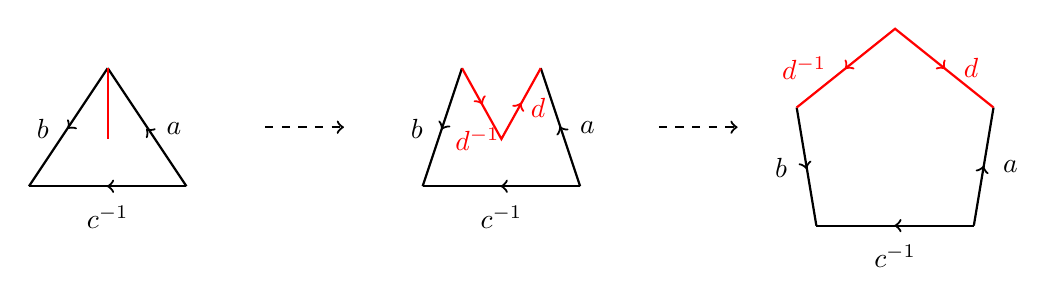
\begin{tikzpicture}
        \shorthandoff{>}
        \begin{scope}[shift={(-5,0)}]
            % Triángulo
            \draw[thick] (1,1.5) -- (0,0); %1
            \draw[thick] (0,0) -- (2,0); %2
            \draw[thick] (2,0) -- (1,1.5); %3

            \draw[red, thick] (1,1.5) -- (1,0.6);

            % Leyenda
            \node[label=left:{$b$}] at (0.5,0.73) {}; %1
            \node[label=below:{$c^{-1}$}] at (1, 0) {}; %2
            \node[label=right:{$a$}] at (1.5, 0.73) {}; %3

            % Flechas
            \draw[->, thick] (0.5,0.73) ++(0, 0.01) -- ++(-0.01,-0.01); %1
            \draw[<-, thick] (1,0) ++(-0.01,0) -- ++(0.01,0); %2
            \draw[->, thick] (1.5,0.73) ++(0, -0.01) -- ++(-0.01,0.01); %3
        \end{scope}

        \draw[dashed, thick, ->] (-2,0.75) -- (-1,0.75);
        
        \begin{scope}[shift={(0,0)}]
            % Triángulo
            \draw[thick] (0.5,1.5) -- (0,0); %1
            \draw[thick] (0,0) -- (2,0); %2
            \draw[thick] (2,0) -- (1.5,1.5); %3

            \draw[red, thick] (0.5,1.5) -- (1,0.6) -- (1.5, 1.5);

            % Leyenda
            \node[label=left:{$b$}] at (0.25,0.73) {}; %1
            \node[label=below:{$c^{-1}$}] at (1, 0) {}; %2
            \node[label=right:{$a$}] at (1.75, 0.75) {}; %3

            \node[label={[red]left:{$d^{-1}$}}, anchor=west] at (1.1, 0.6) {};
            \node[label={[red]right:{$d$}}, anchor=east] at (1.25, 1) {};

            % Flechas
            \draw[->, thick] (0.25,0.73) ++(0, 0.01) -- ++(-0.01,-0.02); %1
            \draw[<-, thick] (1,0) ++(-0.01,0) -- ++(0.01,0); %2
            \draw[->, thick] (1.75, 0.75) ++(0, -0.01) -- ++(-0.01,0.02); %3

            \draw[<-, thick, red] (0.75, 1.05) ++(0.01,-0.01) -- ++(-0.01,0.02); %2
            \draw[->, thick, red] (1.25, 1.05) ++(-0.01,-0.01) -- ++(0.01,0.02); %3
        \end{scope}

        \draw[dashed, thick, ->] (3,0.75) -- (4,0.75);
        
        \begin{scope}[shift={(5,-0.5)}]
            % Triángulo
            \draw[thick] (-0.25,1.5) -- (0,0); %1
            \draw[thick] (0,0) -- (2,0); %2
            \draw[thick] (2,0) -- (2.25,1.5); %3

            \draw[red, thick] (-0.25,1.5) -- (1,2.5) -- (2.25, 1.5);

            % Leyenda
            \node[label=left:{$b$}] at (-0.125,0.73) {}; %1
            \node[label=below:{$c^{-1}$}] at (1, 0) {}; %2
            \node[label=right:{$a$}] at (2.125, 0.75) {}; %3

            \node[label={[red]left:{$d^{-1}$}}] at (0.375, 2) {};
            \node[label={[red]right:{$d$}}] at (1.625, 2) {};

            % Flechas
            \draw[<-, thick] (-0.125,0.73) ++(0, -0.01) -- ++(-0.01,0.04); %1
            \draw[<-, thick] (1,0) ++(-0.01,0) -- ++(0.01,0); %2
            \draw[<-, thick] (2.125, 0.75) ++(0, 0.01) -- ++(-0.01,-0.04); %3

            \draw[<-, thick, red] (0.375, 2) ++(-0.01,-0.01) -- ++(0.01,0.01); %2
            \draw[<-, thick, red] (1.625, 2) ++(0.01,-0.01) -- ++(-0.01,0.01); %3
        \end{scope}

    \end{tikzpicture}
\end{figure}

\subsubsection{Doblar}
Es el proceso contrario a desdoblar. Si una expresión $w$ tiene de forma consecutiva un símbolo y el mismo con exponente cambiado podemos quitar dicho símbolo de la expresión. Esto se podrá hacer siempre que al quitarle estos símbolos queden al menos 3.

\begin{figure}[H]
    \centering
    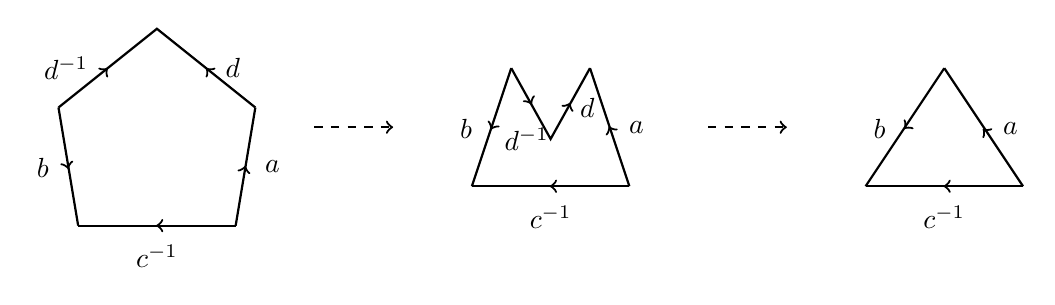
\begin{tikzpicture}
        \shorthandoff{>}
        \begin{scope}[shift={(-5,-0.5)}]
            % Triángulo
            \draw[thick] (-0.25,1.5) -- (0,0); %1
            \draw[thick] (0,0) -- (2,0); %2
            \draw[thick] (2,0) -- (2.25,1.5); %3

            \draw[thick] (-0.25,1.5) -- (1,2.5) -- (2.25, 1.5);

            % Leyenda
            \node[label=left:{$b$}] at (-0.125,0.73) {}; %1
            \node[label=below:{$c^{-1}$}] at (1, 0) {}; %2
            \node[label=right:{$a$}] at (2.125, 0.75) {}; %3

            \node[label={left:{$d^{-1}$}}] at (0.375, 2) {};
            \node[label={right:{$d$}}] at (1.625, 2) {};

            % Flechas
            \draw[<-, thick] (-0.125,0.73) ++(0, -0.01) -- ++(-0.01,0.04); %1
            \draw[<-, thick] (1,0) ++(-0.01,0) -- ++(0.01,0); %2
            \draw[<-, thick] (2.125, 0.75) ++(0, 0.01) -- ++(-0.01,-0.04); %3

            \draw[->, thick] (0.375, 2) ++(-0.01,-0.01) -- ++(0.01,0.01); %2
            \draw[->, thick] (1.625, 2) ++(0.01,-0.01) -- ++(-0.01,0.01); %3
        \end{scope}

        \draw[dashed, thick, ->] (-2,0.75) -- (-1,0.75);
        
        \begin{scope}[shift={(0,0)}]
            % Triángulo
            \draw[thick] (0.5,1.5) -- (0,0); %1
            \draw[thick] (0,0) -- (2,0); %2
            \draw[thick] (2,0) -- (1.5,1.5); %3

            \draw[thick] (0.5,1.5) -- (1,0.6) -- (1.5, 1.5);

            % Leyenda
            \node[label=left:{$b$}] at (0.25,0.73) {}; %1
            \node[label=below:{$c^{-1}$}] at (1, 0) {}; %2
            \node[label=right:{$a$}] at (1.75, 0.75) {}; %3

            \node[label={left:{$d^{-1}$}}, anchor=west] at (1.1, 0.6) {};
            \node[label={right:{$d$}}, anchor=east] at (1.25, 1) {};

            % Flechas
            \draw[->, thick] (0.25,0.73) ++(0, 0.01) -- ++(-0.01,-0.02); %1
            \draw[<-, thick] (1,0) ++(-0.01,0) -- ++(0.01,0); %2
            \draw[->, thick] (1.75, 0.75) ++(0, -0.01) -- ++(-0.01,0.02); %3

            \draw[<-, thick] (0.75, 1.05) ++(0.01,-0.01) -- ++(-0.01,0.02); %2
            \draw[->, thick] (1.25, 1.05) ++(-0.01,-0.01) -- ++(0.01,0.02); %3
        \end{scope}

        \draw[dashed, thick, ->] (3,0.75) -- (4,0.75);
        
        \begin{scope}[shift={(5,0)}]
            % Triángulo
            \draw[thick] (1,1.5) -- (0,0); %1
            \draw[thick] (0,0) -- (2,0); %2
            \draw[thick] (2,0) -- (1,1.5); %3

            % Leyenda
            \node[label=left:{$b$}] at (0.5,0.73) {}; %1
            \node[label=below:{$c^{-1}$}] at (1, 0) {}; %2
            \node[label=right:{$a$}] at (1.5, 0.73) {}; %3

            % Flechas
            \draw[->, thick] (0.5,0.73) ++(0, 0.01) -- ++(-0.01,-0.01); %1
            \draw[<-, thick] (1,0) ++(-0.01,0) -- ++(0.01,0); %2
            \draw[->, thick] (1.5,0.73) ++(0, -0.01) -- ++(-0.01,0.01); %3
        \end{scope}
    \end{tikzpicture}
\end{figure}

\begin{ejemplo}\ 
    \begin{enumerate}
        \item Consideramos la presentación $\cc{P} = \{a,b,c\ ; a^{-1}cb,\ ac^{-1}b^{-1}\}$. Veamos qué superficie $|\cc{P}|$ tiene asociada. De la presentación podemos obtener los triángulos $w_1=a^{-1}cb$ y $w_2=ac^{-1b^{-1}}$.
         
        \begin{figure}[H]
            \centering
            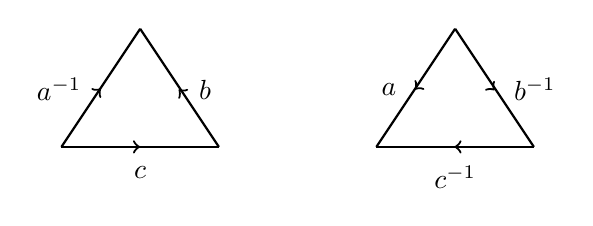
\begin{tikzpicture}
                \shorthandoff{>}
                
                \begin{scope}[shift={(-2,0)}]
                    % Triángulo
                    \draw[thick] (1,1.5) -- (0,0); %1
                    \draw[thick] (0,0) -- (2,0); %2
                    \draw[thick] (2,0) -- (1,1.5); %3

                    % Leyenda
                    \node[label=left:{$a^{-1}$}] at (0.5,0.73) {}; %1
                    \node[label=below:{$c$}] at (1, 0) {}; %2
                    \node[label=right:{$b$}] at (1.5, 0.73) {}; %3

                    % Flechas
                    \draw[<-, thick] (0.5,0.73) ++(0, 0.01) -- ++(-0.01,-0.01); %1
                    \draw[->, thick] (1,0) ++(-0.01,0) -- ++(0.01,0); %2
                    \draw[->, thick] (1.5,0.73) ++(0, -0.01) -- ++(-0.01,0.01); %3
                \end{scope}

                \begin{scope}[shift={(2,0)}]
                    % Triángulo
                    \draw[thick] (1,1.5) -- (0,0); %1
                    \draw[thick] (0,0) -- (2,0); %2
                    \draw[thick] (2,0) -- (1,1.5); %3

                    % Leyenda
                    \node[label=left:{$a$}] at (0.5,0.73) {}; %1
                    \node[label=below:{$c^{-1}$}] at (1, 0) {}; %2
                    \node[label=right:{$b^{-1}$}] at (1.5, 0.73) {}; %3

                    % Flechas
                    \draw[->, thick] (0.5,0.73) ++(0, 0.01) -- ++(-0.01,-0.01); %1
                    \draw[<-, thick] (1,0) ++(-0.01,0) -- ++(0.01,0); %2
                    \draw[<-, thick] (1.5,0.73) ++(0, -0.01) -- ++(-0.01,0.01); %3
                \end{scope}
            \end{tikzpicture}
        \end{figure}

        Podemos ahora rotar $w_1$ y $w_2$ obteniendo $w_1'=ba^{-1}c$ y $w_2'=c^{-1}b^{-1}a$.

        \begin{figure}[H]
            \centering
            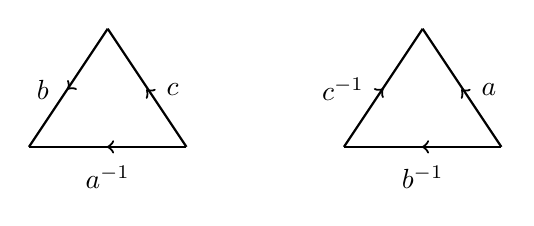
\begin{tikzpicture}
                \shorthandoff{>}
                
                \begin{scope}[shift={(-2,0)}]
                    % Triángulo
                    \draw[thick] (1,1.5) -- (0,0); %1
                    \draw[thick] (0,0) -- (2,0); %2
                    \draw[thick] (2,0) -- (1,1.5); %3

                    % Leyenda
                    \node[label=left:{$b$}] at (0.5,0.73) {}; %1
                    \node[label=below:{$a^{-1}$}] at (1, 0) {}; %2
                    \node[label=right:{$c$}] at (1.5, 0.73) {}; %3

                    % Flechas
                    \draw[->, thick] (0.5,0.73) ++(0, 0.01) -- ++(-0.01,-0.01); %1
                    \draw[<-, thick] (1,0) ++(-0.01,0) -- ++(0.01,0); %2
                    \draw[->, thick] (1.5,0.73) ++(0, -0.01) -- ++(-0.01,0.01); %3
                \end{scope}

                \begin{scope}[shift={(2,0)}]
                    % Triángulo
                    \draw[thick] (1,1.5) -- (0,0); %1
                    \draw[thick] (0,0) -- (2,0); %2
                    \draw[thick] (2,0) -- (1,1.5); %3

                    % Leyenda
                    \node[label=left:{$c^{-1}$}] at (0.5,0.73) {}; %1
                    \node[label=below:{$b^{-1}$}] at (1, 0) {}; %2
                    \node[label=right:{$a$}] at (1.5, 0.73) {}; %3

                    % Flechas
                    \draw[<-, thick] (0.5,0.73) ++(0, 0.01) -- ++(-0.01,-0.01); %1
                    \draw[<-, thick] (1,0) ++(-0.01,0) -- ++(0.01,0); %2
                    \draw[->, thick] (1.5,0.73) ++(0, -0.01) -- ++(-0.01,0.01); %3
                \end{scope}
            \end{tikzpicture}
        \end{figure}

        Estamos ahora en condiciones de pegar ambos triángulos a través de $c$ obteniendo $w_0=ba^{-1}b^{-1}a$.

        \begin{figure}[H]
            \centering
            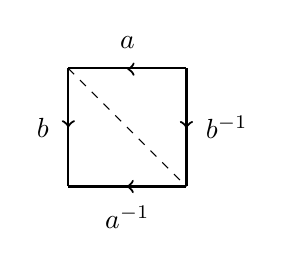
\begin{tikzpicture}
                \shorthandoff{>}
                % Cuadrado
                \draw[thick] (0,1.5) -- (0,0); %1
                \draw[thick] (0,0) -- (1.5,0); %2
                \draw[thick] (1.5,0) -- (1.5,1.5); %3
                \draw[thick] (1.5,1.5) -- (0,1.5); %4

                \draw[dashed] (0,1.5) -- (1.5,0);

                % Leyenda
                \node[label=left:{$b$}] at (0, 0.75) {}; %1
                \node[label=below:{$a^{-1}$}] at (0.75, 0) {}; %2
                \node[label=right:{$b^{-1}$}] at (1.5, 0.75) {}; %3
                \node[label=above:{$a$}] at (0.75, 1.5) {}; %4

                % Flechas
                \draw[->, thick] (0,0.75) ++(0, 0.01) -- ++(0,-0.01); %1
                \draw[<-, thick] (0.75,0) ++(-0.01,0) -- ++(0.01,0); %2
                \draw[<-, thick] (1.5,0.75) ++(0, -0.01) -- ++(0,0.01); %3
                \draw[->, thick] (0.75,1.5) ++(0.01, -0.01) -- ++(-0.01,0); %4
            \end{tikzpicture}
        \end{figure}

        Con una última rotación obtenemos $w_0'=aba^{-1}b^{-1}$ que es fácil ver que se corresponde a un toro.

        \begin{figure}[H]
            \centering
            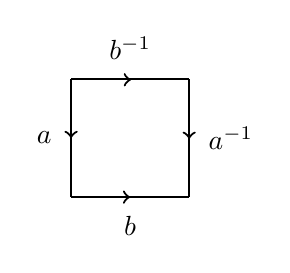
\begin{tikzpicture}
                \shorthandoff{>}
                % Cuadrado
                \draw[thick] (0,1.5) -- (0,0); %1
                \draw[thick] (0,0) -- (1.5,0); %2
                \draw[thick] (1.5,0) -- (1.5,1.5); %3
                \draw[thick] (1.5,1.5) -- (0,1.5); %4

                % Leyenda
                \node[label=left:{$a$}] at (0, 0.75) {}; %1
                \node[label=below:{$b$}] at (0.75, 0) {}; %2
                \node[label=right:{$a^{-1}$}] at (1.5, 0.75) {}; %3
                \node[label=above:{$b^{-1}$}] at (0.75, 1.5) {}; %4

                % Flechas
                \draw[->, thick] (0,0.75) ++(0, 0.01) -- ++(0,-0.01); %1
                \draw[->, thick] (0.75,0) ++(-0.01,0) -- ++(0.01,0); %2
                \draw[<-, thick] (1.5,0.75) ++(0, -0.01) -- ++(0,0.01); %3
                \draw[<-, thick] (0.75,1.5) ++(0.01, -0.01) -- ++(-0.01,0); %4
            \end{tikzpicture}
        \end{figure}

        Podemos resumir todo el proceso como
        \begin{gather*}
            a^{-1}cb,\ ac^{-1}b^{-1} \sim ba^{-1}c,\ c^{-1}b^{-1}a \sim ba^{-1}b^{-1}a \sim aba^{-1}b^{-1}
        \end{gather*}
        Obtenemos entonces $|\cc{P}|\equiv \bb{T}$.

        \item $\cc{P}=\{a,b\ ;aabb\}$. Partimos por tanto de $w_0=aabb$.
        
        \begin{figure}[H]
            \centering
            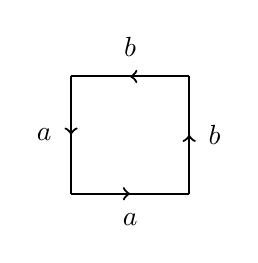
\begin{tikzpicture}
                \shorthandoff{>}
                % Cuadrado
                \draw[thick] (0,1.5) -- (0,0); %1
                \draw[thick] (0,0) -- (1.5,0); %2
                \draw[thick] (1.5,0) -- (1.5,1.5); %3
                \draw[thick] (1.5,1.5) -- (0,1.5); %4

                % Leyenda
                \node[label=left:{$a$}] at (0, 0.75) {}; %1
                \node[label=below:{$a$}] at (0.75, 0) {}; %2
                \node[label=right:{$b$}] at (1.5, 0.75) {}; %3
                \node[label=above:{$b$}] at (0.75, 1.5) {}; %4

                % Flechas
                \draw[->, thick] (0,0.75) ++(0, 0.01) -- ++(0,-0.01); %1
                \draw[->, thick] (0.75,0) ++(-0.01,0) -- ++(0.01,0); %2
                \draw[->, thick] (1.5,0.75) ++(0, -0.01) -- ++(0,0.01); %3
                \draw[->, thick] (0.75,1.5) ++(0.01, -0.01) -- ++(-0.01,0); %4
            \end{tikzpicture}
        \end{figure}

        Le aplicamos una rotación para obtener $w_0'=abba$.

        \begin{figure}[H]
            \centering
            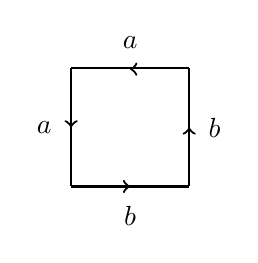
\begin{tikzpicture}
                \shorthandoff{>}
                % Cuadrado
                \draw[thick] (0,1.5) -- (0,0); %1
                \draw[thick] (0,0) -- (1.5,0); %2
                \draw[thick] (1.5,0) -- (1.5,1.5); %3
                \draw[thick] (1.5,1.5) -- (0,1.5); %4

                % Leyenda
                \node[label=left:{$a$}] at (0, 0.75) {}; %1
                \node[label=below:{$b$}] at (0.75, 0) {}; %2
                \node[label=right:{$b$}] at (1.5, 0.75) {}; %3
                \node[label=above:{$a$}] at (0.75, 1.5) {}; %4

                % Flechas
                \draw[->, thick] (0,0.75) ++(0, 0.01) -- ++(0,-0.01); %1
                \draw[->, thick] (0.75,0) ++(-0.01,0) -- ++(0.01,0); %2
                \draw[->, thick] (1.5,0.75) ++(0, -0.01) -- ++(0,0.01); %3
                \draw[->, thick] (0.75,1.5) ++(0.01, -0.01) -- ++(-0.01,0); %4
            \end{tikzpicture}
        \end{figure}

        Podemos ahora cortar obteniendo $w_1=abc$ y $w_2=c^{-1}ba$.

        \begin{figure}[H]
            \centering
            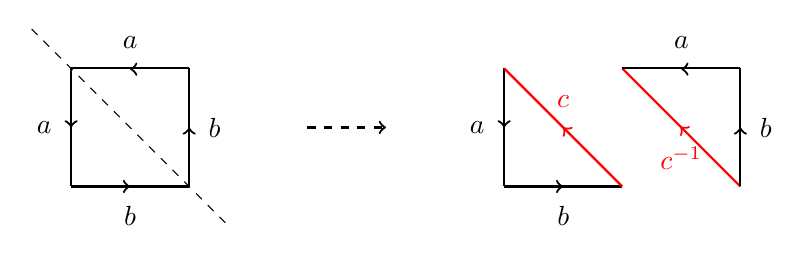
\begin{tikzpicture}
                \shorthandoff{>}
                \begin{scope}[shift={(-3.5,0)}]
                    % Cuadrado
                    \draw[thick] (0,1.5) -- (0,0); %1
                    \draw[thick] (0,0) -- (1.5,0); %2
                    \draw[thick] (1.5,0) -- (1.5,1.5); %3
                    \draw[thick] (1.5,1.5) -- (0,1.5); %4

                    \draw[dashed] (-0.5,2) -- (2,-0.5);

                    % Leyenda
                    \node[label=left:{$a$}] at (0, 0.75) {}; %1
                    \node[label=below:{$b$}] at (0.75, 0) {}; %2
                    \node[label=right:{$b$}] at (1.5, 0.75) {}; %3
                    \node[label=above:{$a$}] at (0.75, 1.5) {}; %4

                    % Flechas
                    \draw[->, thick] (0,0.75) ++(0, 0.01) -- ++(0,-0.01); %1
                    \draw[->, thick] (0.75,0) ++(-0.01,0) -- ++(0.01,0); %2
                    \draw[->, thick] (1.5,0.75) ++(0, -0.01) -- ++(0,0.01); %3
                    \draw[->, thick] (0.75,1.5) ++(0.01, -0.01) -- ++(-0.01,0); %4
                \end{scope}

                \draw[thick, dashed, ->] (-0.5,0.75) -- (0.5,0.75);

                \begin{scope}[shift={(2,0)}]
                    % Cuadrado
                    \draw[thick] (0,1.5) -- (0,0); %1
                    \draw[thick] (0,0) -- (1.5,0); %2
                    \draw[thick, red] (1.5,0) -- (0,1.5); %3-4

                    % Leyenda
                    \node[label=left:{$a$}] at (0, 0.75) {}; %1
                    \node[label=below:{$b$}] at (0.75, 0) {}; %2
                    \node[label={[red]above:{$c$}}] at (0.75, 0.75) {}; %3-4

                    % Flechas
                    \draw[->, thick] (0,0.75) ++(0, 0.01) -- ++(0,-0.01); %1
                    \draw[->, thick] (0.75,0) ++(-0.01,0) -- ++(0.01,0); %2
                    \draw[->, thick, red] (0.75,0.75) ++(0.01, -0.01) -- ++(-0.01,0.01); %3-4
                \end{scope}

                \begin{scope}[shift={(3.5,0)}]
                    % Cuadrado
                    \draw[thick, red] (1.5,0) -- (0,1.5); %1-2
                    \draw[thick] (1.5,0) -- (1.5,1.5); %3
                    \draw[thick] (1.5,1.5) -- (0,1.5); %4

                    % Leyenda
                    \node[label={[red]below:{$c^{-1}$}}] at (0.75, 0.75) {}; %1-2
                    \node[label=right:{$b$}] at (1.5, 0.75) {}; %3
                    \node[label=above:{$a$}] at (0.75, 1.5) {}; %4

                    % Flechas
                    \draw[<-, thick, red] (0.75,0.75) ++(-0.01, 0.01) -- ++(0.01,-0.01); %1-2
                    \draw[->, thick] (1.5,0.75) ++(0, -0.01) -- ++(0,0.01); %3
                    \draw[->, thick] (0.75,1.5) ++(0.01, -0.01) -- ++(-0.01,0); %4
                \end{scope}
            \end{tikzpicture}
        \end{figure}

        Aplicamos ahora una simetría a $w_2$ obteniendo $w_2'=a^{-1}b^{-1}c$

        \begin{figure}[H]
            \centering
            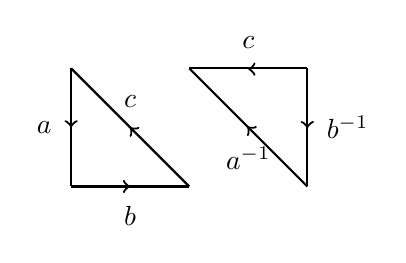
\begin{tikzpicture}
                \shorthandoff{>}
                \begin{scope}[shift={(2,0)}]
                    % Cuadrado
                    \draw[thick] (0,1.5) -- (0,0); %1
                    \draw[thick] (0,0) -- (1.5,0); %2
                    \draw[thick] (1.5,0) -- (0,1.5); %3-4

                    % Leyenda
                    \node[label=left:{$a$}] at (0, 0.75) {}; %1
                    \node[label=below:{$b$}] at (0.75, 0) {}; %2
                    \node[label={above:{$c$}}] at (0.75, 0.75) {}; %3-4

                    % Flechas
                    \draw[->, thick] (0,0.75) ++(0, 0.01) -- ++(0,-0.01); %1
                    \draw[->, thick] (0.75,0) ++(-0.01,0) -- ++(0.01,0); %2
                    \draw[->, thick] (0.75,0.75) ++(0.01, -0.01) -- ++(-0.01,0.01); %3-4
                \end{scope}

                \begin{scope}[shift={(3.5,0)}]
                    % Cuadrado
                    \draw[thick] (1.5,0) -- (0,1.5); %1-2
                    \draw[thick] (1.5,0) -- (1.5,1.5); %3
                    \draw[thick] (1.5,1.5) -- (0,1.5); %4

                    % Leyenda
                    \node[label={below:{$a^{-1}$}}] at (0.75, 0.75) {}; %1-2
                    \node[label=right:{$b^{-1}$}] at (1.5, 0.75) {}; %3
                    \node[label=above:{$c$}] at (0.75, 1.5) {}; %4

                    % Flechas
                    \draw[<-, thick] (0.75,0.75) ++(-0.01, 0.01) -- ++(0.01,-0.01); %1-2
                    \draw[<-, thick] (1.5,0.75) ++(0, -0.01) -- ++(0,0.01); %3
                    \draw[->, thick] (0.75,1.5) ++(0.01, -0.01) -- ++(-0.01,0); %4
                \end{scope}
            \end{tikzpicture}
        \end{figure}
        
        Rotamos ambos polígonos para obtener $w_1'=cab$ y $w_2''=b^{-1}ca^{-1}$

        \begin{figure}[H]
            \centering
            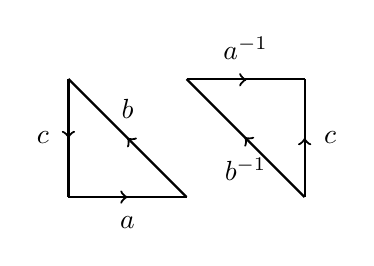
\begin{tikzpicture}
                \shorthandoff{>}
                \begin{scope}[shift={(2,0)}]
                    % Cuadrado
                    \draw[thick] (0,1.5) -- (0,0); %1
                    \draw[thick] (0,0) -- (1.5,0); %2
                    \draw[thick] (1.5,0) -- (0,1.5); %3-4

                    % Leyenda
                    \node[label=left:{$c$}] at (0, 0.75) {}; %1
                    \node[label=below:{$a$}] at (0.75, 0) {}; %2
                    \node[label={above:{$b$}}] at (0.75, 0.75) {}; %3-4

                    % Flechas
                    \draw[->, thick] (0,0.75) ++(0, 0.01) -- ++(0,-0.01); %1
                    \draw[->, thick] (0.75,0) ++(-0.01,0) -- ++(0.01,0); %2
                    \draw[->, thick] (0.75,0.75) ++(0.01, -0.01) -- ++(-0.01,0.01); %3-4
                \end{scope}

                \begin{scope}[shift={(3.5,0)}]
                    % Cuadrado
                    \draw[thick] (1.5,0) -- (0,1.5); %1-2
                    \draw[thick] (1.5,0) -- (1.5,1.5); %3
                    \draw[thick] (1.5,1.5) -- (0,1.5); %4

                    % Leyenda
                    \node[label={below:{$b^{-1}$}}] at (0.75, 0.75) {}; %1-2
                    \node[label=right:{$c$}] at (1.5, 0.75) {}; %3
                    \node[label=above:{$a^{-1}$}] at (0.75, 1.5) {}; %4

                    % Flechas
                    \draw[<-, thick] (0.75,0.75) ++(-0.01, 0.01) -- ++(0.01,-0.01); %1-2
                    \draw[->, thick] (1.5,0.75) ++(0, -0.01) -- ++(0,0.01); %3
                    \draw[<-, thick] (0.75,1.5) ++(0.01, -0.01) -- ++(-0.01,0); %4
                \end{scope}
            \end{tikzpicture}
        \end{figure}

        Finalmente podemos pegar ambos triángulos por $b$ obteniendo $w_0''=caca^{-1}$

        \begin{figure}[H]
            \centering
            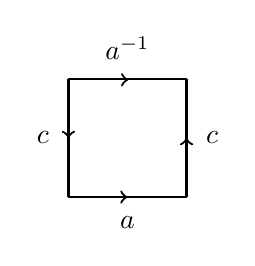
\begin{tikzpicture}
                \shorthandoff{>}
                % Cuadrado
                \draw[thick] (0,1.5) -- (0,0); %1
                \draw[thick] (0,0) -- (1.5,0); %2
                \draw[thick] (1.5,0) -- (1.5,1.5); %3
                \draw[thick] (1.5,1.5) -- (0,1.5); %4

                % Leyenda
                \node[label=left:{$c$}] at (0, 0.75) {}; %1
                \node[label=below:{$a$}] at (0.75, 0) {}; %2
                \node[label=right:{$c$}] at (1.5, 0.75) {}; %3
                \node[label=above:{$a^{-1}$}] at (0.75, 1.5) {}; %4

                % Flechas
                \draw[->, thick] (0,0.75) ++(0, 0.01) -- ++(0,-0.01); %1
                \draw[->, thick] (0.75,0) ++(-0.01,0) -- ++(0.01,0); %2
                \draw[->, thick] (1.5,0.75) ++(0, -0.01) -- ++(0,0.01); %3
                \draw[<-, thick] (0.75,1.5) ++(0.01, -0.01) -- ++(-0.01,0); %4
            \end{tikzpicture}
        \end{figure}

        Podemos resumir todo el proceso como
        \begin{gather*}
            aabb \sim abba \sim abc,\ c^{-1}ba \sim abc,\ a^{-1}b^{-1}c \sim cab,\ b^{-1}ca^{-1} \sim caca^{-1}
        \end{gather*}
        La expresión final es $caca^{-1}$ que intuitivamente corresponde a la botella de Klein. Para ver esto tenemos que pensar en identificar inicialmente el lado $a$ con $a^{-1}$ lo que crearía un cilindro. Si ahora identificáramos los extremos de forma directa tendríamos un toro (que es el ejemplo anterior) pero tenemos que se unen de manera inversa. Esto haría que tuviese que "atravesarse a sí mismo" y al unirse con el otro extremo llegaríamos a la botella de Klein.

        \item $\cc{P}=\{a,b\ ;aa^{-1}bb\}$. Partimos de $w_0=aa^{-1}bb$.
        \begin{figure}[H]
            \centering
            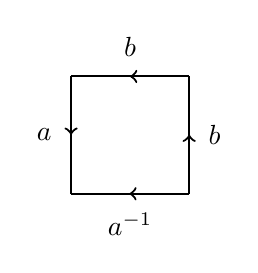
\begin{tikzpicture}
                \shorthandoff{>}
                % Cuadrado
                \draw[thick] (0,1.5) -- (0,0); %1
                \draw[thick] (0,0) -- (1.5,0); %2
                \draw[thick] (1.5,0) -- (1.5,1.5); %3
                \draw[thick] (1.5,1.5) -- (0,1.5); %4

                % Leyenda
                \node[label=left:{$a$}] at (0, 0.75) {}; %1
                \node[label=below:{$a^{-1}$}] at (0.75, 0) {}; %2
                \node[label=right:{$b$}] at (1.5, 0.75) {}; %3
                \node[label=above:{$b$}] at (0.75, 1.5) {}; %4

                % Flechas
                \draw[->, thick] (0,0.75) ++(0, 0.01) -- ++(0,-0.01); %1
                \draw[<-, thick] (0.75,0) ++(-0.01,0) -- ++(0.01,0); %2
                \draw[->, thick] (1.5,0.75) ++(0, -0.01) -- ++(0,0.01); %3
                \draw[->, thick] (0.75,1.5) ++(0.01, -0.01) -- ++(-0.01,0); %4
            \end{tikzpicture}
        \end{figure}

        Podemos ahora aplicar una rotación obteniendo $w_0'=baa^{-1}b$.

        \begin{figure}[H]
            \centering
            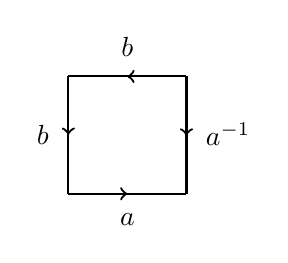
\begin{tikzpicture}
                \shorthandoff{>}
                % Cuadrado
                \draw[thick] (0,1.5) -- (0,0); %1
                \draw[thick] (0,0) -- (1.5,0); %2
                \draw[thick] (1.5,0) -- (1.5,1.5); %3
                \draw[thick] (1.5,1.5) -- (0,1.5); %4

                % Leyenda
                \node[label=left:{$b$}] at (0, 0.75) {}; %1
                \node[label=below:{$a$}] at (0.75, 0) {}; %2
                \node[label=right:{$a^{-1}$}] at (1.5, 0.75) {}; %3
                \node[label=above:{$b$}] at (0.75, 1.5) {}; %4

                % Flechas
                \draw[->, thick] (0,0.75) ++(0, 0.01) -- ++(0,-0.01); %1
                \draw[->, thick] (0.75,0) ++(-0.01,0) -- ++(0.01,0); %2
                \draw[<-, thick] (1.5,0.75) ++(0, -0.01) -- ++(0,0.01); %3
                \draw[->, thick] (0.75,1.5) ++(0.01, -0.01) -- ++(-0.01,0); %4
            \end{tikzpicture}
        \end{figure}

        Cortamos obteniendo $w_1=bac$ y $w_2=c^{-1}a^{-1}b$.

        \begin{figure}[H]
            \centering
            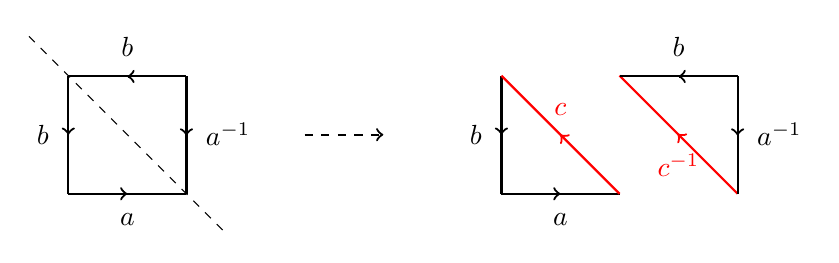
\begin{tikzpicture}
                \shorthandoff{>}
                \begin{scope}[shift={(-3.5,0)}]
                    % Cuadrado
                    \draw[thick] (0,1.5) -- (0,0); %1
                    \draw[thick] (0,0) -- (1.5,0); %2
                    \draw[thick] (1.5,0) -- (1.5,1.5); %3
                    \draw[thick] (1.5,1.5) -- (0,1.5); %4

                    \draw[dashed] (-0.5, 2) -- (2,-0.5);

                    % Leyenda
                    \node[label=left:{$b$}] at (0, 0.75) {}; %1
                    \node[label=below:{$a$}] at (0.75, 0) {}; %2
                    \node[label=right:{$a^{-1}$}] at (1.5, 0.75) {}; %3
                    \node[label=above:{$b$}] at (0.75, 1.5) {}; %4

                    % Flechas
                    \draw[->, thick] (0,0.75) ++(0, 0.01) -- ++(0,-0.01); %1
                    \draw[->, thick] (0.75,0) ++(-0.01,0) -- ++(0.01,0); %2
                    \draw[<-, thick] (1.5,0.75) ++(0, -0.01) -- ++(0,0.01); %3
                    \draw[->, thick] (0.75,1.5) ++(0.01, -0.01) -- ++(-0.01,0); %4
                \end{scope}

                \draw[thick, dashed, ->] (-0.5,0.75) -- (0.5,0.75);

                \begin{scope}[shift={(2,0)}]
                    % Cuadrado
                    \draw[thick] (0,1.5) -- (0,0); %1
                    \draw[thick] (0,0) -- (1.5,0); %2
                    \draw[thick, red] (1.5,0) -- (0,1.5); %3-4

                    % Leyenda
                    \node[label=left:{$b$}] at (0, 0.75) {}; %1
                    \node[label=below:{$a$}] at (0.75, 0) {}; %2
                    \node[label={[red]above:{$c$}}] at (0.75, 0.75) {}; %3-4

                    % Flechas
                    \draw[->, thick] (0,0.75) ++(0, 0.01) -- ++(0,-0.01); %1
                    \draw[->, thick] (0.75,0) ++(-0.01,0) -- ++(0.01,0); %2
                    \draw[->, thick, red] (0.75,0.75) ++(0.01, -0.01) -- ++(-0.01,0.01); %3-4
                \end{scope}

                \begin{scope}[shift={(3.5,0)}]
                    % Cuadrado
                    \draw[thick, red] (1.5,0) -- (0,1.5); %1-2
                    \draw[thick] (1.5,0) -- (1.5,1.5); %3
                    \draw[thick] (1.5,1.5) -- (0,1.5); %4

                    % Leyenda
                    \node[label={[red]below:{$c^{-1}$}}] at (0.75, 0.75) {}; %1-2
                    \node[label=right:{$a^{-1}$}] at (1.5, 0.75) {}; %3
                    \node[label=above:{$b$}] at (0.75, 1.5) {}; %4

                    % Flechas
                    \draw[<-, thick, red] (0.75,0.75) ++(-0.01, 0.01) -- ++(0.01,-0.01); %1-2
                    \draw[<-, thick] (1.5,0.75) ++(0, -0.01) -- ++(0,0.01); %3
                    \draw[->, thick] (0.75,1.5) ++(0.01, -0.01) -- ++(-0.01,0); %4
                \end{scope}
            \end{tikzpicture}
        \end{figure}

        Aplicamos una simetría a $w_2$ obteniendo $w_2'=b^{-1}ac$

        \begin{figure}[H]
            \centering
            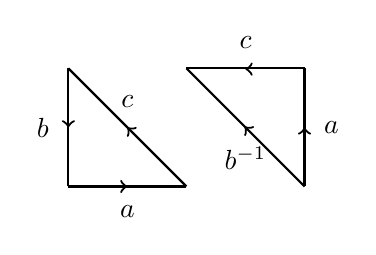
\begin{tikzpicture}
                \shorthandoff{>}
                \begin{scope}[shift={(2,0)}]
                    % Cuadrado
                    \draw[thick] (0,1.5) -- (0,0); %1
                    \draw[thick] (0,0) -- (1.5,0); %2
                    \draw[thick] (1.5,0) -- (0,1.5); %3-4

                    % Leyenda
                    \node[label=left:{$b$}] at (0, 0.75) {}; %1
                    \node[label=below:{$a$}] at (0.75, 0) {}; %2
                    \node[label={above:{$c$}}] at (0.75, 0.75) {}; %3-4

                    % Flechas
                    \draw[->, thick] (0,0.75) ++(0, 0.01) -- ++(0,-0.01); %1
                    \draw[->, thick] (0.75,0) ++(-0.01,0) -- ++(0.01,0); %2
                    \draw[->, thick] (0.75,0.75) ++(0.01, -0.01) -- ++(-0.01,0.01); %3-4
                \end{scope}

                \begin{scope}[shift={(3.5,0)}]
                    % Cuadrado
                    \draw[thick] (1.5,0) -- (0,1.5); %1-2
                    \draw[thick] (1.5,0) -- (1.5,1.5); %3
                    \draw[thick] (1.5,1.5) -- (0,1.5); %4

                    % Leyenda
                    \node[label={below:{$b^{-1}$}}] at (0.75, 0.75) {}; %1-2
                    \node[label=right:{$a$}] at (1.5, 0.75) {}; %3
                    \node[label=above:{$c$}] at (0.75, 1.5) {}; %4

                    % Flechas
                    \draw[<-, thick] (0.75,0.75) ++(-0.01, 0.01) -- ++(0.01,-0.01); %1-2
                    \draw[->, thick] (1.5,0.75) ++(0, -0.01) -- ++(0,0.01); %3
                    \draw[->, thick] (0.75,1.5) ++(0.01, -0.01) -- ++(-0.01,0); %4
                \end{scope}
            \end{tikzpicture}
        \end{figure}

        Rotamos ahora $w_1$ triángulos obteniendo $w_1'=acb$

        \begin{figure}[H]
            \centering
            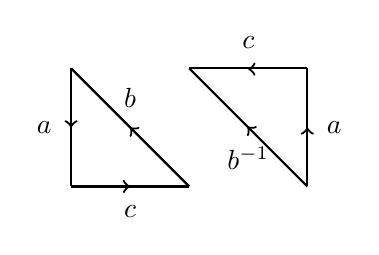
\begin{tikzpicture}
                \shorthandoff{>}
                \begin{scope}[shift={(2,0)}]
                    % Cuadrado
                    \draw[thick] (0,1.5) -- (0,0); %1
                    \draw[thick] (0,0) -- (1.5,0); %2
                    \draw[thick] (1.5,0) -- (0,1.5); %3-4

                    % Leyenda
                    \node[label=left:{$a$}] at (0, 0.75) {}; %1
                    \node[label=below:{$c$}] at (0.75, 0) {}; %2
                    \node[label={above:{$b$}}] at (0.75, 0.75) {}; %3-4

                    % Flechas
                    \draw[->, thick] (0,0.75) ++(0, 0.01) -- ++(0,-0.01); %1
                    \draw[->, thick] (0.75,0) ++(-0.01,0) -- ++(0.01,0); %2
                    \draw[->, thick] (0.75,0.75) ++(0.01, -0.01) -- ++(-0.01,0.01); %3-4
                \end{scope}

                \begin{scope}[shift={(3.5,0)}]
                    % Cuadrado
                    \draw[thick] (1.5,0) -- (0,1.5); %1-2
                    \draw[thick] (1.5,0) -- (1.5,1.5); %3
                    \draw[thick] (1.5,1.5) -- (0,1.5); %4

                    % Leyenda
                    \node[label={below:{$b^{-1}$}}] at (0.75, 0.75) {}; %1-2
                    \node[label=right:{$a$}] at (1.5, 0.75) {}; %3
                    \node[label=above:{$c$}] at (0.75, 1.5) {}; %4

                    % Flechas
                    \draw[<-, thick] (0.75,0.75) ++(-0.01, 0.01) -- ++(0.01,-0.01); %1-2
                    \draw[->, thick] (1.5,0.75) ++(0, -0.01) -- ++(0,0.01); %3
                    \draw[->, thick] (0.75,1.5) ++(0.01, -0.01) -- ++(-0.01,0); %4
                \end{scope}
            \end{tikzpicture}
        \end{figure}

        Unimos finalmente a través de $b$ obteniendo $w_0''=acac$.

        \begin{figure}[H]
            \centering
            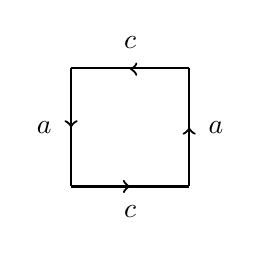
\begin{tikzpicture}
                \shorthandoff{>}
                % Cuadrado
                \draw[thick] (0,1.5) -- (0,0); %1
                \draw[thick] (0,0) -- (1.5,0); %2
                \draw[thick] (1.5,0) -- (1.5,1.5); %3
                \draw[thick] (1.5,1.5) -- (0,1.5); %4

                % Leyenda
                \node[label=left:{$a$}] at (0, 0.75) {}; %1
                \node[label=below:{$c$}] at (0.75, 0) {}; %2
                \node[label=right:{$a$}] at (1.5, 0.75) {}; %3
                \node[label=above:{$c$}] at (0.75, 1.5) {}; %4

                % Flechas
                \draw[->, thick] (0,0.75) ++(0, 0.01) -- ++(0,-0.01); %1
                \draw[->, thick] (0.75,0) ++(-0.01,0) -- ++(0.01,0); %2
                \draw[->, thick] (1.5,0.75) ++(0, -0.01) -- ++(0,0.01); %3
                \draw[->, thick] (0.75,1.5) ++(0.01, -0.01) -- ++(-0.01,0); %4
            \end{tikzpicture}
        \end{figure}

        Podemos resumir el proceso como
        \begin{gather*}
            aa^{-1}bb \sim baa^{-1}b \sim bac,\ c^{-1}a^{-1}b \sim bac,\ b^{-1}ac \sim acb,\ b^{-1}ac \sim acac
        \end{gather*}
        Tenemos que $|\cc{P}|$ es el plano proyectivo $\bb{R}\bb{P}^2$. Para verlo podemos ver la última figura como una circunferencia donde se identifica cada punto del borde con su antípoda.

        \begin{figure}[H]
            \centering
            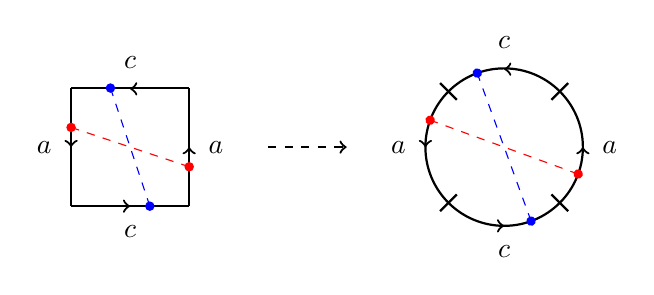
\begin{tikzpicture}
                \shorthandoff{>}
                \begin{scope}[shift={(-3,-0.75)}]
                    % Cuadrado
                    \draw[thick] (0,1.5) -- (0,0); %1
                    \draw[thick] (0,0) -- (1.5,0); %2
                    \draw[thick] (1.5,0) -- (1.5,1.5); %3
                    \draw[thick] (1.5,1.5) -- (0,1.5); %4

                    % Leyenda
                    \node[label=left:{$a$}] at (0, 0.75) {}; %1
                    \node[label=below:{$c$}] at (0.75, 0) {}; %2
                    \node[label=right:{$a$}] at (1.5, 0.75) {}; %3
                    \node[label=above:{$c$}] at (0.75, 1.5) {}; %4

                    % Flechas
                    \draw[->, thick] (0,0.75) ++(0, 0.01) -- ++(0,-0.01); %1
                    \draw[->, thick] (0.75,0) ++(-0.01,0) -- ++(0.01,0); %2
                    \draw[->, thick] (1.5,0.75) ++(0, -0.01) -- ++(0,0.01); %3
                    \draw[->, thick] (0.75,1.5) ++(0.01, -0.01) -- ++(-0.01,0); %4

                    % Identificaciones
                    \filldraw[blue] (0.5,1.5) circle (1.5pt);
                    \filldraw[blue] (1,0) circle (1.5pt);
                    \draw[dashed, blue] (0.5,1.5)--(1,0);

                    \filldraw[red] (0,1) circle (1.5pt);
                    \filldraw[red] (1.5,0.5) circle (1.5pt);
                    \draw[dashed, red] (0,1)--(1.5,0.5);
                \end{scope}

                \draw[dashed, ->, thick] (-0.5,0) -- (0.5, 0);

                \begin{scope}[shift={(2.5,0)}]
                    %Circunferencia
                    \draw[thick] (0,0) circle [radius=1];

                    % Leyenda
                    \node[label=left:{$a$}] at (-1,0) {}; %1
                    \node[label=below:{$c$}] at (0,-1) {}; %2
                    \node[label=right:{$a$}] at (1,0) {}; %3
                    \node[label=above:{$c$}] at (0,1) {}; %4

                    % Flechas
                    \draw[->, thick] (-1,0) ++(0, 0.01) -- ++(0,-0.01); %1
                    \draw[->, thick] (0,-1) ++(-0.01,0) -- ++(0.01,0); %2
                    \draw[->, thick] (1,0) ++(0, -0.01) -- ++(0,0.01); %3
                    \draw[->, thick] (0,1) ++(0.01, -0.01) -- ++(-0.01,0); %4

                    % Separadores
                    \draw[thick, rotate around={45:(0,0)}] (0.85,0) -- (1.15,0);
                    \draw[thick, rotate around={135:(0,0)}] (0.85,0) -- (1.15,0);
                    \draw[thick, rotate around={225:(0,0)}] (0.85,0) -- (1.15,0);
                    \draw[thick, rotate around={315:(0,0)}] (0.85,0) -- (1.15,0);

                    % Identificaciones
                    \filldraw[blue, rotate around={110:(0,0)}] (-1,0) circle (1.5pt);
                    \filldraw[blue, rotate around={110:(0,0)}] (1,0) circle (1.5pt);
                    \draw[dashed, blue, rotate around={110:(0,0)}] (-1,0)--(1,0);

                    \filldraw[red, rotate around={160:(0,0)}] (-1,0) circle (1.5pt);
                    \filldraw[red, rotate around={160:(0,0)}] (1,0) circle (1.5pt);
                    \draw[dashed, red, rotate around={160:(0,0)}] (-1,0)--(1,0);
                \end{scope}
            \end{tikzpicture}
        \end{figure}

    \end{enumerate}   
\end{ejemplo}

\section{La clasificación de las superficies compactas}

\begin{prop}
    Sean $S_1$ y $S_2$ dos superficies compactas dadas respectivamente como $|\cc{P}_1|$ y $|\cc{P}_2|$ para las presentaciones 
    \begin{gather*}
        \cc{P}_1=\{a_1,...,a_n;w_1\}\ \ \text{ y } \ \ \cc{P}_2=\{b_1,...,b_2;w_2\}
    \end{gather*}
    donde cada presentación tiene una única expresión\footnote{esto implica que ambas son conexas}. Entonces $S_1\#S_2$ tiene como presentación 
    \begin{gather*}
        \cc{P}= \{a_1,...,a_n,b_1,...,b_k;w_1w_2\}
    \end{gather*}
\end{prop}

\begin{coro}
    Una presentación de 
    \begin{enumerate}
        \item la esfera es $aa^{-1}bb^{-1}$.
        \item el plano proyectivo es $aa^{-1}bb$.
        \item el $n$-toro o esfera de $n$ asas $\bb{T}_n$ es $a_1b_1a_1^{-1}b_1^{-1}a_2b_2a_2^{-1}b_2^{-1}...a_nb_na_n^{-1}b_n^{-1}$.
        \item el $n$-plano proyectivo $\bb{R}\bb{P}_n^2$ es $a_1a_1a_2a_2...a_na_n$
    \end{enumerate}
    \begin{proof}
        Los casos 1., 2. y 3. son claros (en el caso 3. se puede ver fácilmente usando la proposición anterior). Estudiemos el caso que nos queda. Sabemos que 
        \begin{gather*}
            \bb{R}\bb{P}_n^2 = \bb{R}\bb{P}^2\# \overset{(n)}{...}\# \bb{R}\bb{P}^2
        \end{gather*}
        Usamos que $\bb{R}\bb{P}^2$ tiene por presentación $bcbc$. Por la proposición anterior tenemos que una presentación de $\bb{R}\bb{P}_n^2$ es 
        \begin{gather*}
            b_1c_1b_1c_1b_2c_2b_2c_2...b_nc_nb_nc_n
        \end{gather*}
        Podemos consolidar y llamar $a_i=b_ic_i$ para todo $i\in \{1,...,n\}$ y tendríamos 
        \begin{gather*}
            b_1c_1b_1c_1b_2c_2b_2c_2...b_nc_nb_nc_n \sim a_1a_1a_2a_2...a_na_n
        \end{gather*}
    \end{proof}
\end{coro}

\begin{observacion}
    Del ejemplo anterior y del corolario se deduce que 
    \begin{gather*}
        \bb{R}\bb{P}^2\#\bb{R}\bb{P}^2 = \bb{R}\bb{P}_2^2 \equiv \text{Botella de Klein}
    \end{gather*}
\end{observacion}

\subsection{Determinación de $|\cc{P}|$}
Nuestro objetivo ahora es llegar a que si tenemos una superficie compacta y conexa $S$, entonces tenemos que 
\begin{gather*}
    S \overset{homeo.}{\cong} \left\{
        \begin{array}{l l}
            \bb{S}^2 &: aa^{-1}bb^{-1}\\
            \bb{T}_n &: a_1b_1a_1^{-1}b_1^{-1}a_2b_2a_2^{-1}b_2^{-1}...a_nb_na_n^{-1}b_n^{-1}\\
            \bb{R}\bb{P}^2_n &: a_1a_1a_2a_2...a_na_n
        \end{array}
    \right.
\end{gather*}

Vamos a partir de una presentación poligonal $\cc{P}$ y vamos a ver un algoritmo que nos dirá que la superficie compacta $|\cc{P}|$ en caso de ser conexa será homeomorfa a alguna de las anteriores.

\subsubsection{Algoritmo de determinación de $|\cc{P}|$}
\begin{enumerate}
    \item El primer paso del algoritmo es diferenciar las componentes conexas de la siguiente forma. Tomamos la primera expresión $w_1$ y a esta le pegamos cualquier otra expresión $w_i$ que tenga un símbolo común. Entonces me queda una nueva expresión $w_1'$ a la que le volvemos a aplicar el paso 1 hasta obtener una expresión donde todos sus símbolos tienen a su pareja en esa expresión. Esta expresión dará (en el cociente) una componente conexa de $|\cc{P}|$. Solamente nos fijaremos entonces en estudiar presentaciones poligonales con una única expresión (ya que queremos que sea conexa).

    \item Ahora de nuestra única expresión le eliminamos los símbolos que aparezcan adyacentes con ellos mismos y con distinto exponente (doblaremos siempre que podamos). Esto lo podremos hacer siempre que al eliminar $aa^{-1}$ nos queden al menos 4 símbolos\footnote{ya que en este caso tienen que estar emparejados}. Si no pudiéramos quitar $aa^{-1}$ de $w$ es porque tenemos o $w=aa^{-1}bb$ o bien $w=aa^{-1}bb^{-1}$. En el primer caso tendremos $|\cc{P}|\cong\bb{R}\bb{P}^2$ y en el segundo tendremos $|\cc{P}|\cong\bb{S}^2$.

    \item Si nuestra expresión es de la forma $w=y_1ay_2a$ donde el símbolo $a$ aparece dos veces con el mismo exponente (y los $y_1$, $y_2$ son conjuntos de expresiones cualesquiera contenidas en $w$), entonces podré cambiar $w$ por $w'=y_1y_2^{-1}aa$ donde si $y_2=b_1^{\veps_1}...b_k^{\veps_k}$ entonces $y_2^{-1}=b_k^{-\veps_k}...b_1^{-\veps_1}$.
    \begin{proof}
        Veamos brevemente una demostración de por qué se puede hacer este cambio. Si tenemos nuestra expresión $w=y_1ay_2a$ podemos realizar un corte obteniendo $w_1=y_1ac$ y $w_2=c^{-1}y_2a$. Buscamos ahora pegar a través de $a$ para lo que reflejamos $w_2$ obteniendo $w_2'=a^{-1}y_2^{-1}c$ y rotamos $w_1$ obteniendo $w_1'=cy_1a$. Estamos ya en condiciones de poder pegar $w_1'$ y $w_2'$ a través de $a$ de donde obtenemos una nueva expresión $w_0'=cy_1y_2^{-1}c$. Podemos renombrar $c=a$ y obtenemos $w_0''=ay_1y_2^{-1}a$. Con una última rotación llegamos a $w_0'''=y_1y_2^{-1}aa$ que es lo que queríamos obtener.
    \end{proof}
    En una cantidad finita de pasos la expresión inicial pasa a ser de la forma 
    \begin{gather*}
        w=ya_1a_1a_2a_2...a_ka_k
    \end{gather*}
    donde en $y$ solo aparecen parejas de símbolos con distinto exponente (cada pareja). Además, usando el paso 2., es decir, eliminando las expresiones adyacentes en $y$, podemos suponer además que cada símbolo en $y$ con su pareja no son adyacentes. \\
    
    Podemos entonces hacer algunas transformaciones elementales para cambiar a una expresión $w'=y'a_1a_1...a_ka_k$ de forma que todos los vértices del polígono asociado a $w'$ son el mismo punto en el cociente (en $|\cc{P}|$).

    \begin{proof}
        Supongamos que existen vértices en el polígono asociado a $w$ que no son el mismo punto en el cociente y elegimos $v_0$ un vértice cualquiera y tenemos que en el conjunto $[v_0]$ hay al menos 2 vértices del polígono (ya que en otro caso tendremos que está entre un lado $a$ y otro $a^{-1}$ y podríamos doblar).\\

        Veamos que se pueden hacer transformaciones elementales para quitarle un vértice a $[v_0]$. De esta forma, en una cantidad finita de pasos $[v_0]$ solo tendrá un representante y así estaremos en la situación mencionada previamente y podremos doblar.\\

        Para ello tomamos un lado $a$ cuyo vértice inicial $v_1$ esté en $[v_0]$ y el final $v_2$ no lo esté ($v_1\in [v_0]$, $v_2\notin[v_0]$). Tenemos entonces una situación como la siguiente

        \begin{figure}[H]
            \centering
            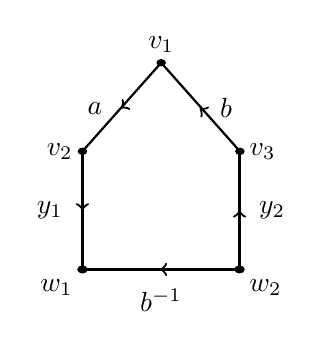
\begin{tikzpicture}
                \shorthandoff{>}
                \begin{scope}[shift={(0,0)}, xscale=1.33]
                    % Cuadrado
                    \draw[thick] (0,1.5) -- (0,0); %1
                    \draw[thick] (0,0) -- (1.5,0); %2
                    \draw[thick] (1.5,0) -- (1.5,1.5); %3
                    % \draw[thick] (1.5,1.5) -- (0,1.5); %4

                    % Leyenda
                    \node[label=left:{$y_1$}] at (0, 0.75) {}; %1
                    \node[label=below:{$b^{-1}$}] at (0.75, 0) {}; %2
                    \node[label=right:{$y_2$}] at (1.5, 0.75) {}; %3
                    % \node[label=above:{$a$}] at (0.75, 1.5) {}; %4

                    % Flechas
                    \draw[->, thick] (0,0.75) ++(0, 0.01) -- ++(0,-0.01); %1
                    \draw[<-, thick] (0.75,0) ++(-0.01,0) -- ++(0.01,0); %2
                    \draw[->, thick] (1.5,0.75) ++(0, -0.01) -- ++(0,0.01); %3
                    % \draw[->, thick] (0.75,1.5) ++(0.01, -0.01) -- ++(-0.01,0); %4

                    % Vértices
                    \filldraw (0,0) circle (1.25pt) node[below left] {$w_1$};
                    \filldraw (1.5,0) circle (1.25pt) node[below right] {$w_2$};
                \end{scope}
                \begin{scope}[shift={(0,1.5)}, yscale=0.75]
                    % Triángulo
                    \draw[thick] (1,1.5) -- (0,0); %1
                    % \draw[thick] (0,0) -- (2,0); %2
                    \draw[thick] (2,0) -- (1,1.5); %3

                    % Leyenda
                    \node[label=left:{$a$}] at (0.5,0.73) {}; %1
                    % \node[label=below:{$a^{-1}$}] at (1, 0) {}; %2
                    \node[label=right:{$b$}] at (1.5, 0.73) {}; %3

                    % Flechas
                    \draw[->, thick] (0.5,0.73) ++(0, 0.01) -- ++(-0.01,-0.01); %1
                    % \draw[<-, thick] (1,0) ++(-0.01,0) -- ++(0.01,0); %2
                    \draw[->, thick] (1.5,0.73) ++(0, -0.01) -- ++(-0.01,0.01); %3

                    % Vértices
                    \filldraw (1,1.5) circle (1.5pt) node[above] {$v_1$};
                    \filldraw (0,0) circle (1.5pt) node[left] {$v_2$};
                    \filldraw (2,0) circle (1.5pt) node[right] {$v_3$};
                \end{scope}
            \end{tikzpicture}
        \end{figure}

        Donde tendremos que $w_1\in [v_0]$ por ser el final de $b^{-1}$ y $v_1$ el final de $b$. Tendremos además que $v_3\in [v_0]$ si y solo si $w_2\in [v_0]$ por ser el principio de $b$ y el de $b^{-1}$ respectivamente. Por tanto $[v_0]$ tendrá o 2 o 4 elementos. Podemos ahora hacer un corte de la siguiente forma:

        \begin{figure}[H]
            \centering
            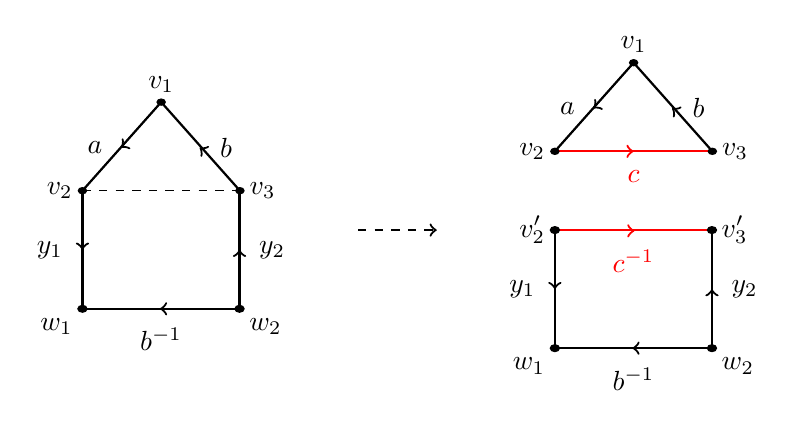
\begin{tikzpicture}
                \shorthandoff{>}
                \begin{scope}[shift={(-4,-1)}]
                   \begin{scope}[shift={(0,0)}, xscale=1.33]
                        % Cuadrado
                        \draw[thick] (0,1.5) -- (0,0); %1
                        \draw[thick] (0,0) -- (1.5,0); %2
                        \draw[thick] (1.5,0) -- (1.5,1.5); %3
                        % \draw[thick] (1.5,1.5) -- (0,1.5); %4

                        % Leyenda
                        \node[label=left:{$y_1$}] at (0, 0.75) {}; %1
                        \node[label=below:{$b^{-1}$}] at (0.75, 0) {}; %2
                        \node[label=right:{$y_2$}] at (1.5, 0.75) {}; %3
                        % \node[label=above:{$a$}] at (0.75, 1.5) {}; %4

                        % Flechas
                        \draw[->, thick] (0,0.75) ++(0, 0.01) -- ++(0,-0.01); %1
                        \draw[<-, thick] (0.75,0) ++(-0.01,0) -- ++(0.01,0); %2
                        \draw[->, thick] (1.5,0.75) ++(0, -0.01) -- ++(0,0.01); %3
                        % \draw[->, thick] (0.75,1.5) ++(0.01, -0.01) -- ++(-0.01,0); %4

                        % Vértices
                        \filldraw (0,0) circle (1.25pt) node[below left] {$w_1$};
                        \filldraw (1.5,0) circle (1.25pt) node[below right] {$w_2$};
                    \end{scope}
                    \begin{scope}[shift={(0,1.5)}, yscale=0.75]
                        % Triángulo
                        \draw[thick] (1,1.5) -- (0,0); %1
                        \draw[dashed] (0,0) -- (2,0); %2
                        \draw[thick] (2,0) -- (1,1.5); %3

                        % Leyenda
                        \node[label=left:{$a$}] at (0.5,0.73) {}; %1
                        % \node[label=below:{$a^{-1}$}] at (1, 0) {}; %2
                        \node[label=right:{$b$}] at (1.5, 0.73) {}; %3

                        % Flechas
                        \draw[->, thick] (0.5,0.73) ++(0, 0.01) -- ++(-0.01,-0.01); %1
                        % \draw[<-, thick] (1,0) ++(-0.01,0) -- ++(0.01,0); %2
                        \draw[->, thick] (1.5,0.73) ++(0, -0.01) -- ++(-0.01,0.01); %3

                        % Vértices
                        \filldraw (1,1.5) circle (1.5pt) node[above] {$v_1$};
                        \filldraw (0,0) circle (1.5pt) node[left] {$v_2$};
                        \filldraw (2,0) circle (1.5pt) node[right] {$v_3$};
                    \end{scope} 
                \end{scope}

                \draw[dashed, thick, ->] (-0.5,0) -- (0.5,0);
                
                \begin{scope}[shift={(2,-1.5)}]
                   \begin{scope}[shift={(0,0)}, xscale=1.33]
                        % Cuadrado
                        \draw[thick] (0,1.5) -- (0,0); %1
                        \draw[thick] (0,0) -- (1.5,0); %2
                        \draw[thick] (1.5,0) -- (1.5,1.5); %3
                        \draw[thick, red] (1.5,1.5) -- (0,1.5); %4

                        % Leyenda
                        \node[label=left:{$y_1$}] at (0, 0.75) {}; %1
                        \node[label=below:{$b^{-1}$}] at (0.75, 0) {}; %2
                        \node[label=right:{$y_2$}] at (1.5, 0.75) {}; %3
                        \node[label={[red]below:{$c^{-1}$}}] at (0.75, 1.5) {}; %4

                        % Flechas
                        \draw[->, thick] (0,0.75) ++(0, 0.01) -- ++(0,-0.01); %1
                        \draw[<-, thick] (0.75,0) ++(-0.01,0) -- ++(0.01,0); %2
                        \draw[->, thick] (1.5,0.75) ++(0, -0.01) -- ++(0,0.01); %3
                        \draw[<-, red, thick] (0.75,1.5) ++(0.01, -0.01) -- ++(-0.01,0); %4

                        % Vértices
                        \filldraw (0,0) circle (1.25pt) node[below left] {$w_1$};
                        \filldraw (1.5,0) circle (1.25pt) node[below right] {$w_2$};
                        \filldraw (1.5,1.5) circle (1.25pt) node[right] {$v_3'$};
                        \filldraw (0,1.5) circle (1.25pt) node[left] {$v_2'$};
                    \end{scope}
                    \begin{scope}[shift={(0,2.5)}, yscale=0.75]
                        % Triángulo
                        \draw[thick] (1,1.5) -- (0,0); %1
                        \draw[thick, red] (0,0) -- (2,0); %2
                        \draw[thick] (2,0) -- (1,1.5); %3

                        % Leyenda
                        \node[label=left:{$a$}] at (0.5,0.73) {}; %1
                        \node[label={[red]below:{$c$}}] at (1, 0) {}; %2
                        \node[label=right:{$b$}] at (1.5, 0.73) {}; %3

                        % Flechas
                        \draw[->, thick] (0.5,0.73) ++(0, 0.01) -- ++(-0.01,-0.01); %1
                        \draw[->, thick, red] (1,0) ++(-0.01,0) -- ++(0.01,0); %2
                        \draw[->, thick] (1.5,0.73) ++(0, -0.01) -- ++(-0.01,0.01); %3

                        % Vértices
                        \filldraw (1,1.5) circle (1.5pt) node[above] {$v_1$};
                        \filldraw (0,0) circle (1.5pt) node[left] {$v_2$};
                        \filldraw (2,0) circle (1.5pt) node[right] {$v_3$};
                    \end{scope} 
                \end{scope}
            \end{tikzpicture}
        \end{figure}

        Podemos ahora colocar convenientemente las piezas (rotando el triángulo que nos queda superiormente y colocándolo debajo del cuadrado) para poder pegar a través de $b$ de la siguiente forma:

        \begin{figure}[H]
            \centering
            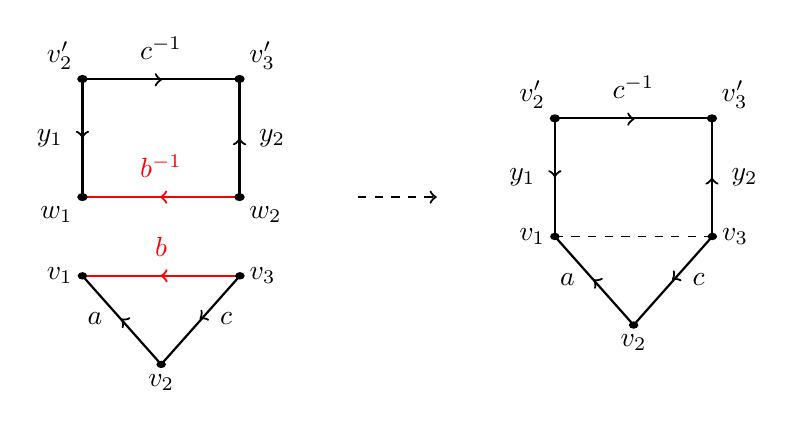
\begin{tikzpicture}
                \shorthandoff{>}
                \begin{scope}[shift={(-4,-1)}]
                   \begin{scope}[shift={(0,1)}, xscale=1.33]
                        % Cuadrado
                        \draw[thick] (0,1.5) -- (0,0); %1
                        \draw[thick, red] (0,0) -- (1.5,0); %2
                        \draw[thick] (1.5,0) -- (1.5,1.5); %3
                        \draw[thick] (1.5,1.5) -- (0,1.5); %4

                        % Leyenda
                        \node[label=left:{$y_1$}] at (0, 0.75) {}; %1
                        \node[label={[red]above:{$b^{-1}$}}] at (0.75, 0) {}; %2
                        \node[label=right:{$y_2$}] at (1.5, 0.75) {}; %3
                        \node[label=above:{$c^{-1}$}] at (0.75, 1.5) {}; %4

                        % Flechas
                        \draw[->, thick] (0,0.75) ++(0, 0.01) -- ++(0,-0.01); %1
                        \draw[<-, thick, red] (0.75,0) ++(-0.01,0) -- ++(0.01,0); %2
                        \draw[->, thick] (1.5,0.75) ++(0, -0.01) -- ++(0,0.01); %3
                        \draw[<-, thick] (0.75,1.5) ++(0.01, -0.01) -- ++(-0.01,0); %4

                        % Vértices
                        \filldraw (0,0) circle (1.25pt) node[below left] {$w_1$};
                        \filldraw (1.5,0) circle (1.25pt) node[below right] {$w_2$};
                        \filldraw (1.5,1.5) circle (1.25pt) node[above right] {$v_3'$};
                        \filldraw (0,1.5) circle (1.25pt) node[above left] {$v_2'$};
                    \end{scope}
                    \begin{scope}[shift={(0,0)}, yscale=0.75]
                        % Triángulo
                        \draw[thick] (1,-1.5) -- (0,0); %1
                        \draw[thick, red] (0,0) -- (2,0); %2
                        \draw[thick] (2,0) -- (1,-1.5); %3

                        % Leyenda
                        \node[label=left:{$a$}] at (0.5,-0.73) {}; %1
                        \node[label={[red]above:{$b$}}] at (1, 0) {}; %2
                        \node[label=right:{$c$}] at (1.5, -0.73) {}; %3

                        % Flechas
                        \draw[->, thick] (0.5,-0.73) ++(0, -0.01) -- ++(-0.01,0.01); %1
                        \draw[<-, thick, red] (1,0) ++(-0.01,0) -- ++(0.01,0); %2
                        \draw[->, thick] (1.5,-0.73) ++(0, 0.01) -- ++(-0.01,-0.01); %3

                        % Vértices
                        \filldraw (1,-1.5) circle (1.5pt) node[below] {$v_2$};
                        \filldraw (0,0) circle (1.5pt) node[left] {$v_1$};
                        \filldraw (2,0) circle (1.5pt) node[right] {$v_3$};
                    \end{scope} 
                \end{scope}

                \draw[dashed, thick, ->] (-0.5,0) -- (0.5,0);
                
                \begin{scope}[shift={(2,-1)}]
                    \begin{scope}[shift={(0,0.5)}, xscale=1.33]
                        % Cuadrado
                        \draw[thick] (0,1.5) -- (0,0); %1
                        % \draw[thick, red] (0,0) -- (1.5,0); %2
                        \draw[thick] (1.5,0) -- (1.5,1.5); %3
                        \draw[thick] (1.5,1.5) -- (0,1.5); %4

                        % Leyenda
                        \node[label=left:{$y_1$}] at (0, 0.75) {}; %1
                        % \node[label={[red]above:{$b^{-1}$}}] at (0.75, 0) {}; %2
                        \node[label=right:{$y_2$}] at (1.5, 0.75) {}; %3
                        \node[label=above:{$c^{-1}$}] at (0.75, 1.5) {}; %4

                        % Flechas
                        \draw[->, thick] (0,0.75) ++(0, 0.01) -- ++(0,-0.01); %1
                        % \draw[<-, thick, red] (0.75,0) ++(-0.01,0) -- ++(0.01,0); %2
                        \draw[->, thick] (1.5,0.75) ++(0, -0.01) -- ++(0,0.01); %3
                        \draw[<-, thick] (0.75,1.5) ++(0.01, -0.01) -- ++(-0.01,0); %4

                        % Vértices
                        % \filldraw (0,0) circle (1.25pt) node[below left] {$w_1$};
                        % \filldraw (1.5,0) circle (1.25pt) node[below right] {$w_2$};
                        \filldraw (1.5,1.5) circle (1.25pt) node[above right] {$v_3'$};
                        \filldraw (0,1.5) circle (1.25pt) node[above left] {$v_2'$};
                    \end{scope}
                    \begin{scope}[shift={(0,0.5)}, yscale=0.75]
                        % Triángulo
                        \draw[thick] (1,-1.5) -- (0,0); %1
                        \draw[dashed] (0,0) -- (2,0); %2
                        \draw[thick] (2,0) -- (1,-1.5); %3

                        % Leyenda
                        \node[label=left:{$a$}] at (0.5,-0.73) {}; %1
                        % \node[label={[red]above:{$b$}}] at (1, 0) {}; %2
                        \node[label=right:{$c$}] at (1.5, -0.73) {}; %3

                        % Flechas
                        \draw[->, thick] (0.5,-0.73) ++(0, -0.01) -- ++(-0.01,0.01); %1
                        % \draw[<-, thick, red] (1,0) ++(-0.01,0) -- ++(0.01,0); %2
                        \draw[->, thick] (1.5,-0.73) ++(0, 0.01) -- ++(-0.01,-0.01); %3

                        % Vértices
                        \filldraw (1,-1.5) circle (1.5pt) node[below] {$v_2$};
                        \filldraw (0,0) circle (1.5pt) node[left] {$v_1$};
                        \filldraw (2,0) circle (1.5pt) node[right] {$v_3$};
                    \end{scope} 
                \end{scope}
            \end{tikzpicture}
        \end{figure}

        En este polígono final tendremos que $v_1\in[v_0]$ y $v_2\notin[v_0]$. Además tendremos que $v_2'\in [v_2]$ por lo que $v_2'\notin[v_0]$ y $v_3'\in [v_3]$. Tenemos ahora que estudiar los dos casos mencionados anteriormente:
        \begin{itemize}
            \item Si $v_3\notin[v_0]$ tendríamos al principio que $[v_0]$ tenía 2 elementos y ahora tiene 1.
            \item Si $v_3\in [v_0]$ tendríamos al principio que $[v_0]$ tenía 4 elementos y ahora tiene 3.
        \end{itemize}

        Por tanto, en este proceso para el nuevo polígono hay un vértice menos en $[v_0]$. Aplicando este proceso un número finito de veces podremos llegar a la siguiente situación:
        \begin{gather*}
            w=ya_1a_1...a_ka_k
        \end{gather*}
        donde solo hay un vértice en el cociente $[v_0]$.
        \begin{itemize}
            \item Si $y=\emptyset$, entonces tendríamos $|\cc{P}|\overset{homeo.}{\cong} \bb{R}\bb{P}^2_k$.
            \item Si $y\neq \emptyset$, entonces en $y$ aparecen aristas con un exponente y su opuesto y, además de forma no adyacente. Debe ocurrir entonces que 
            \begin{gather*}
                y=...\ b\ ...\ c\ ...\ b^{-1}...\ c^{-1}...
            \end{gather*}
        \end{itemize}
    \end{proof}
    \item Si tenemos una expresión del tipo 
    \begin{gather*}
        w = y_1by_2cy_3b^{-1}y_4c^{-1}y_5a_1a_1...a_ka_k
    \end{gather*}
    entonces, cortando y pegando podemos pasar a una expresión del tipo
    \begin{gather*}
        w'=ybcb^{-1}c^{-1}a_1a_1...a_ka_k
    \end{gather*}
    En un proceso finito nos quedará:
    \begin{gather*}
        w''=b_1c_1b_1^{-1}c_1^{-1}...\ b_lc_lb_l^{-1}c_l^{-1}a_1a_1...a_ka_k
    \end{gather*}

    \item Las expresiones del tipo $ybcb^{-1}c^{-1}aa$ las podemos cambiar por transformaciones elementales por 
    \begin{gather*}
        y'aabbcc
    \end{gather*}
\end{enumerate}

Como conclusión final, la expresión inicial se puede alterar haciendo transformaciones elementales del tipo
\begin{enumerate}
    \item $aa^{-1}b^{-1} \equiv \bb{S}^2$.
    \item $aa^{-1}bb \equiv \bb{R}\bb{P}^2$.
    \item $a_1a_1...a_ka_k \equiv \bb{R}\bb{P}_k^{2}$ para $k\geq 2$.
    \item $b_1c_1b_1^{-1}c_1^{-1}...\ b_lc_lc_l^{-1}c_l^{-1} \equiv \bb{T}_l$.
\end{enumerate}

\begin{coro}
    Si $S$ es una superficie compacta (y conexa) entonces $S$ es homeomorfa a $\bb{S}^2$, al $n$-toro o al $k$-plano proyectivo (para $k\geq 1$).
\end{coro}

Veamos ahora que todas esas superficies son distintas calculando su grupo fundamental. Ya conocemos los siguientes:
\begin{gather*}
    \begin{array}{c c c c}
        \bb{S}^2 & \longrightarrow & \pi_1(\bb{S}^2) & \equiv \text{trivial}\\
        \bb{R}\bb{P}^2 & \longrightarrow & \pi_1(\bb{R}\bb{P}^2) & \equiv \bb{Z}_2
    \end{array}
\end{gather*}
Calculemos el grupo fundamental del $n$-toro.

\begin{figure}[H]
    \centering
    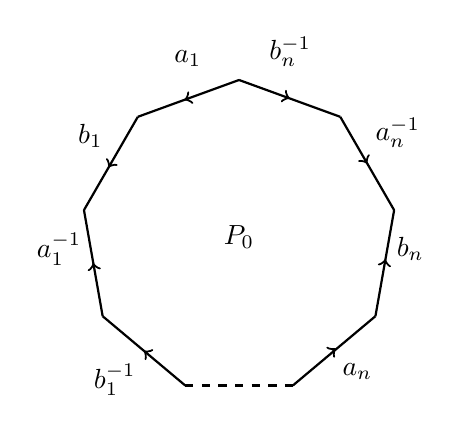
\begin{tikzpicture}
        \shorthandoff{>}

        % \draw[thick]
        % ( 0.6840, -1.8794) --
        % ( 1.7321, -1.0000) --
        % ( 1.9696,  0.3473) --
        % ( 1.2856,  1.5321) --
        % ( 0.0000,  2.0000) --
        % (-1.2856,  1.5321) --
        % (-1.9696,  0.3473) --
        % (-1.7321, -1.0000) --
        % (-0.6840, -1.8794) -- cycle;

        % Lado 1
        \draw[thick] ( 0.6840, -1.8794) -- ( 1.7321, -1.0000);
        \draw[thick,->] ( 1.1880, -1.4397) -- ( 1.2280, -1.4097);
        \node at (1.19, -1.48) [below right] {$a_n$};

        % Lado 2
        \draw[thick] ( 1.7321, -1.0000) -- ( 1.9696,  0.3473);
        \draw[thick,->] ( 1.8509, -0.3264) -- ( 1.8589, -0.2764);
        \node at (1.88, -0.15) [right] {$b_n$};

        % Lado 3
        \draw[thick] ( 1.9696,  0.3473) -- ( 1.2856,  1.5321);
        \draw[thick,<-] ( 1.6276,  0.9397) -- ( 1.5976,  0.9897);
        \node at (1.61, 1.02) [above right] {$a_n^{-1}$};

        % Lado 4
        \draw[thick] ( 1.2856,  1.5321) -- ( 0.0000,  2.0000);
        \draw[thick,<-] ( 0.6428,  1.7660) -- ( 0.5928,  1.7860);
        \node at (0.65, 2.05) [above] {$b_n^{-1}$};

        % Lado 5
        \draw[thick] ( 0.0000,  2.0000) -- (-1.2856,  1.5321);
        \draw[thick,->] (-0.6428,  1.7660) -- (-0.6928,  1.7460);
        \node at (-0.65, 2.05) [above] {$a_1$};

        % Lado 6
        \draw[thick] (-1.2856,  1.5321) -- (-1.9696,  0.3473);
        \draw[thick,->] (-1.6276,  0.9397) -- (-1.6576,  0.8897);
        \node at (-1.61, 1.02) [above left] {$b_1$};

        % Lado 7
        \draw[thick] (-1.9696,  0.3473) -- (-1.7321, -1.0000);
        \draw[thick,<-] (-1.8509, -0.3264) -- (-1.8429, -0.3764);
        \node at (-1.88, -0.15) [left] {$a_1^{-1}$};

        % Lado 8
        \draw[thick] (-1.7321, -1.0000) -- (-0.6840, -1.8794);
        \draw[thick,<-] (-1.2080, -1.4397) -- (-1.1680, -1.4697);
        \node at (-1.19, -1.48) [below left] {$b_1^{-1}$};

        % Lado 9
        \draw[dashed, thick] (-0.6840, -1.8794) -- ( 0.6840, -1.8794);
        % \draw[thick,->] ( 0.0000, -1.8794) -- ( 0.0500, -1.8794);
        % \node at (0, -1.92) [below] {L9};

        \node at (0,0) {$P_0$};
    \end{tikzpicture}
\end{figure}

Este será $P_0$ bajo la relación de equivalencia $R$ que identifica a los lados con igual nombre, es decir
\begin{gather*}
    \bb{T}_n = \frac{P_0}{R}
\end{gather*}
Buscamos aplicar Seifert-van Kampen y tomamos 
\begin{gather*}
    U=\bb{T}_n \setminus \{x_0\}\\
    V \equiv \text{ disco abierto centrado en $x_0$ que no toque las aristas}
\end{gather*}

\begin{figure}[H]
    \centering
    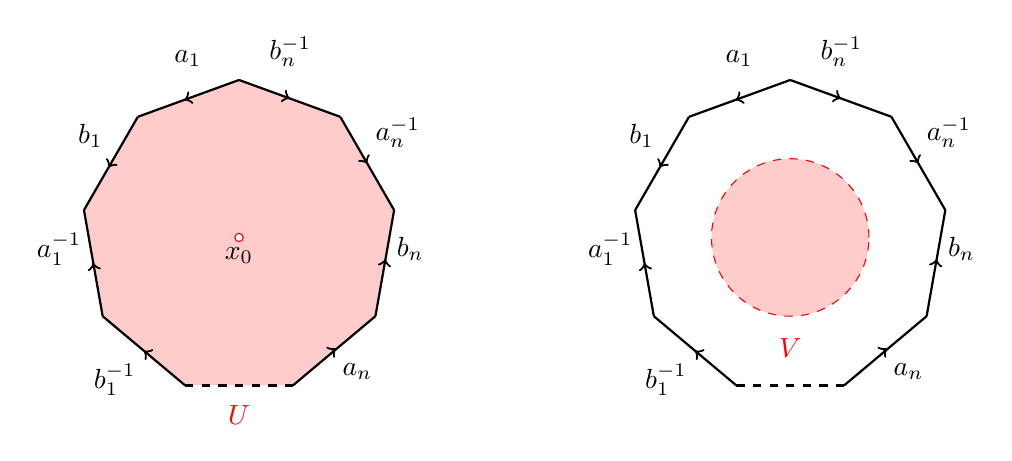
\begin{tikzpicture}
        \shorthandoff{>}
        \begin{scope}

            \fill[red!20]
                ( 0.6840, -1.8794) --
                ( 1.7321, -1.0000) --
                ( 1.9696,  0.3473) --
                ( 1.2856,  1.5321) --
                ( 0.0000,  2.0000) --
                (-1.2856,  1.5321) --
                (-1.9696,  0.3473) --
                (-1.7321, -1.0000) --
                (-0.6840, -1.8794) -- cycle;
            % Lado 1
            \draw[thick] ( 0.6840, -1.8794) -- ( 1.7321, -1.0000);
            \draw[thick,->] ( 1.1880, -1.4397) -- ( 1.2280, -1.4097);
            \node at (1.19, -1.48) [below right] {$a_n$};

            % Lado 2
            \draw[thick] ( 1.7321, -1.0000) -- ( 1.9696,  0.3473);
            \draw[thick,->] ( 1.8509, -0.3264) -- ( 1.8589, -0.2764);
            \node at (1.88, -0.15) [right] {$b_n$};

            % Lado 3
            \draw[thick] ( 1.9696,  0.3473) -- ( 1.2856,  1.5321);
            \draw[thick,<-] ( 1.6276,  0.9397) -- ( 1.5976,  0.9897);
            \node at (1.61, 1.02) [above right] {$a_n^{-1}$};

            % Lado 4
            \draw[thick] ( 1.2856,  1.5321) -- ( 0.0000,  2.0000);
            \draw[thick,<-] ( 0.6428,  1.7660) -- ( 0.5928,  1.7860);
            \node at (0.65, 2.05) [above] {$b_n^{-1}$};

            % Lado 5
            \draw[thick] ( 0.0000,  2.0000) -- (-1.2856,  1.5321);
            \draw[thick,->] (-0.6428,  1.7660) -- (-0.6928,  1.7460);
            \node at (-0.65, 2.05) [above] {$a_1$};

            % Lado 6
            \draw[thick] (-1.2856,  1.5321) -- (-1.9696,  0.3473);
            \draw[thick,->] (-1.6276,  0.9397) -- (-1.6576,  0.8897);
            \node at (-1.61, 1.02) [above left] {$b_1$};

            % Lado 7
            \draw[thick] (-1.9696,  0.3473) -- (-1.7321, -1.0000);
            \draw[thick,<-] (-1.8509, -0.3264) -- (-1.8429, -0.3764);
            \node at (-1.88, -0.15) [left] {$a_1^{-1}$};

            % Lado 8
            \draw[thick] (-1.7321, -1.0000) -- (-0.6840, -1.8794);
            \draw[thick,<-] (-1.2080, -1.4397) -- (-1.1680, -1.4697);
            \node at (-1.19, -1.48) [below left] {$b_1^{-1}$};

            % Lado 9
            \draw[dashed, thick] (-0.6840, -1.8794) -- ( 0.6840, -1.8794);
            % \draw[thick,->] ( 0.0000, -1.8794) -- ( 0.0500, -1.8794);
            % \node at (0, -1.92) [below] {L9};

            \filldraw[fill=white, draw=red] (0,0) circle (1.5pt) node[below] {$x_0$};
            \node[red] at (0,-2.25) {$U$};
        \end{scope}
        \begin{scope}[shift={(7,0)}]
            % Lado 1
            \draw[thick] ( 0.6840, -1.8794) -- ( 1.7321, -1.0000);
            \draw[thick,->] ( 1.1880, -1.4397) -- ( 1.2280, -1.4097);
            \node at (1.19, -1.48) [below right] {$a_n$};

            % Lado 2
            \draw[thick] ( 1.7321, -1.0000) -- ( 1.9696,  0.3473);
            \draw[thick,->] ( 1.8509, -0.3264) -- ( 1.8589, -0.2764);
            \node at (1.88, -0.15) [right] {$b_n$};

            % Lado 3
            \draw[thick] ( 1.9696,  0.3473) -- ( 1.2856,  1.5321);
            \draw[thick,<-] ( 1.6276,  0.9397) -- ( 1.5976,  0.9897);
            \node at (1.61, 1.02) [above right] {$a_n^{-1}$};

            % Lado 4
            \draw[thick] ( 1.2856,  1.5321) -- ( 0.0000,  2.0000);
            \draw[thick,<-] ( 0.6428,  1.7660) -- ( 0.5928,  1.7860);
            \node at (0.65, 2.05) [above] {$b_n^{-1}$};

            % Lado 5
            \draw[thick] ( 0.0000,  2.0000) -- (-1.2856,  1.5321);
            \draw[thick,->] (-0.6428,  1.7660) -- (-0.6928,  1.7460);
            \node at (-0.65, 2.05) [above] {$a_1$};

            % Lado 6
            \draw[thick] (-1.2856,  1.5321) -- (-1.9696,  0.3473);
            \draw[thick,->] (-1.6276,  0.9397) -- (-1.6576,  0.8897);
            \node at (-1.61, 1.02) [above left] {$b_1$};

            % Lado 7
            \draw[thick] (-1.9696,  0.3473) -- (-1.7321, -1.0000);
            \draw[thick,<-] (-1.8509, -0.3264) -- (-1.8429, -0.3764);
            \node at (-1.88, -0.15) [left] {$a_1^{-1}$};

            % Lado 8
            \draw[thick] (-1.7321, -1.0000) -- (-0.6840, -1.8794);
            \draw[thick,<-] (-1.2080, -1.4397) -- (-1.1680, -1.4697);
            \node at (-1.19, -1.48) [below left] {$b_1^{-1}$};

            % Lado 9
            \draw[dashed, thick] (-0.6840, -1.8794) -- ( 0.6840, -1.8794);
            % \draw[thick,->] ( 0.0000, -1.8794) -- ( 0.0500, -1.8794);
            % \node at (0, -1.92) [below] {L9};

            %V
            \filldraw[dashed, fill=red!20, draw=red] (0,0) circle [radius=1cm];
            \node[red] at (0,-1.4) {$V$};
        \end{scope}
    \end{tikzpicture}
\end{figure}

Es claro que $\pi_1(V)$ es trivial por ser un disco. Para calcular el grupo fundamental de $U$ comenzamos considerando un retracto de deformación suyo. Es fácil ver que el borde (en el cociente) es retracto de deformación de $U$. Además, todos los vértices del borde tendrán la misma clase de equivalencia bajo $R$. Para ver esto último vamos a numerar los vértices como $v_{ij}$ con $i\in \{1,...,4\}$ y $j\in \{1,...,n\}$ de forma que $v_{1j}$ sea el principio de $a_j$, $v_{2j}$ el principio de $b_j$, $v_{3j}$ será el principio de $a_j^{-1}$ y $v_{4j}$ será el principio de $b_j^{-1}$ para todo $j\in \{1,...,n\}$. Es decir,

\begin{figure}[H]
    \centering
    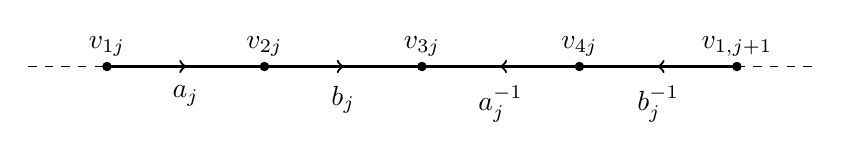
\begin{tikzpicture}
        \shorthandoff{>}
        % Línea
        \draw[dashed] (-5,0) -- (-4,0);
        \draw[thick] (-4,0) -- (4,0);
        \draw[dashed] (4,0) -- (5,0);

        % Vértices
        \filldraw (-4,0) circle (1.5pt) node[above] {$v_{1j}$};
        \filldraw (-2,0) circle (1.5pt) node[above] {$v_{2j}$};
        \filldraw (0,0) circle (1.5pt) node[above] {$v_{3j}$};
        \filldraw (2,0) circle (1.5pt) node[above] {$v_{4j}$};
        \filldraw (4,0) circle (1.5pt) node[above] {$v_{1,j+1}$};

        % Flechas
        \draw[thick,->] (-3.01,0) -- (-2.99,0);
        \draw[thick,->] (-1.01,0) -- (-0.99,0);
        \draw[thick,<-] (0.99,0) -- (1.01,0);
        \draw[thick,<-] (2.99,0) -- (3.01,0);

        % Lados
        \node[label=below:{$a_j$}] at (-3,0) {};
        \node[label=below:{$b_j$}] at (-1,0) {};
        \node[label=below:{$a_j^{-1}$}] at (1,0) {};
        \node[label=below:{$b_j^{-1}$}] at (3,0) {};
    \end{tikzpicture}
\end{figure}

Entonces tenemos que 
\begin{gather*}
    [v_{1j}] = [v_{4j}] \text{ por ser principio de $a_j$ y $a_j^{-1}$ respectivamente}\\
    [v_{4j}] = [v_{3j}] \text{ por ser final de $b_j^{-1}$ y $b_j$ respectivamente}\\
    [v_{3j}] = [v_{2j}] \text{ por ser final de $a_j^{-1}$ y $a_j$ respectivamente}\\
    [v_{2j}] = [v_{1,j+1}] \text{ por ser principio de $b_j$ y $b_j^{-1}$ respectivamente}\\
\end{gather*}
Como la $j$ es arbitraria se verificará para todo $j\in\{1,...,n\}$ (entendiendo que $n+1$ vuelve a ser el $1$) y por tanto todos los vértices son de la misma clase de equivalencia. Nos quedará algo como 

\begin{figure}[H]
    \centering
    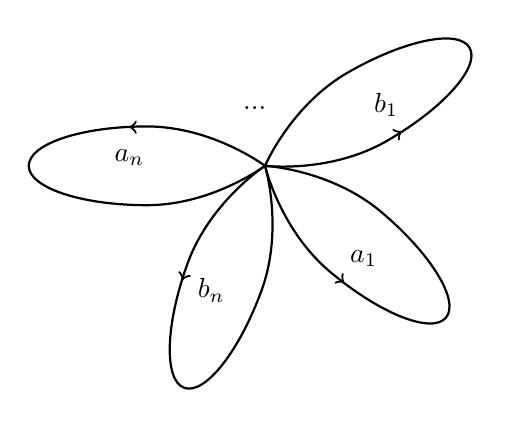
\begin{tikzpicture}
        \shorthandoff{>}
        \begin{scope}
            \draw[thick] plot[smooth, tension=1] coordinates {
                (0,0) (-1.5,0.5) (-3,0) (-1.5,-0.5) (0,0)
            };
            \draw[->, thick] (-1.72,0.49) ++(+0.01, 0) -- ++(-0.01,0);
            \node at (-1.72, 0.1) {$a_n$};
        \end{scope}

        \begin{scope}[rotate around={70:(0,0)}]
            \draw[thick] plot[smooth, tension=1] coordinates {
                (0,0) (-1.5,0.5) (-3,0) (-1.5,-0.5) (0,0)
            };
            \draw[->, thick] (-1.72,0.49) ++(+0.01, 0) -- ++(-0.01,0);
            \node at (-1.72, 0.1) {$b_n$};
        \end{scope}

        \begin{scope}[rotate around={140:(0,0)}]
            \draw[thick] plot[smooth, tension=1] coordinates {
                (0,0) (-1.5,0.5) (-3,0) (-1.5,-0.5) (0,0)
            };
            \draw[->, thick] (-1.72,0.49) ++(+0.01, 0) -- ++(-0.01,0);
            \node at (-1.72, 0.1) {$a_1$};
        \end{scope}

        \begin{scope}[rotate around={210:(0,0)}]
            \draw[thick] plot[smooth, tension=1] coordinates {
                (0,0) (-1.5,0.5) (-3,0) (-1.5,-0.5) (0,0)
            };
            \draw[->, thick] (-1.72,0.49) ++(+0.01, 0) -- ++(-0.01,0);
            \node at (-1.72, 0.1) {$b_1$};
        \end{scope}

        \begin{scope}[rotate around={280:(0,0)}]
            \node at (-0.75, 0) {$...$};
        \end{scope}
    \end{tikzpicture}%
\end{figure}%

por lo que $\pi_1(U)\cong F(a_1,b_1,a_2,b_2,...,a_n,b_n)$. Además el grupo de la intersección es claro que es $\pi_1(U\cap V) \cong \bb{Z}$ generado por $[\alpha]$ ya que tiene a una circunferencia centrada en $x_0$ y de radio menor que el radio de $V$ por retracto de deformación.

\begin{figure}[H]
    \centering
    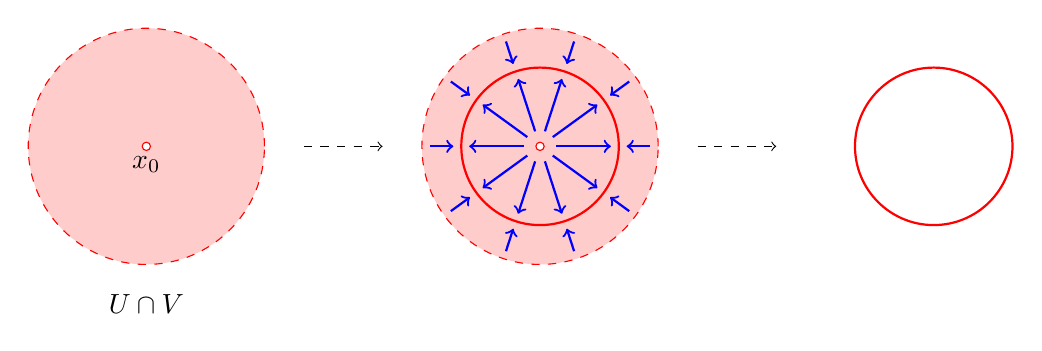
\begin{tikzpicture}
        \begin{scope} [shift={(-5,0)}]
            \filldraw[fill=red!20, draw=red, dashed] (0,0) circle [radius=1.5cm];
            \filldraw[fill=white, draw=red] (0,0) circle (1.5pt) node[below] {$x_0$};
            \node at (0,-2) {$U\cap V$};
        \end{scope}

        \draw[dashed, ->] (-3,0) -- (-2,0);

        \begin{scope}
            \filldraw[fill=red!20, draw=red, dashed] (0,0) circle [radius=1.5cm];
            \filldraw[fill=white, draw=red] (0,0) circle (1.5pt);

            \draw[red, thick] (0,0) circle [radius=1cm];

            % Flechas
            \def\n{10}
            \foreach \i in {0,...,\numexpr\n-1\relax} {
                \draw[thick, blue, ->] ({360/\n * \i}:0.2) -- ({360/\n * \i}:0.9);
                \draw[thick, blue, ->] ({360/\n * \i}:1.4) -- ({360/\n * \i}:1.1);
            }
        \end{scope}

        \draw[dashed, ->] (2,0) -- (3,0);

        \begin{scope}[shift={(5,0)}]
            \draw[red, thick] (0,0) circle [radius=1cm];
        \end{scope}
    \end{tikzpicture}
\end{figure}

Aplicando Seifert-van Kampen tenemos que 
\begin{gather*}
    \pi_1(\bb{T}_n) = \frac{F(a_1,b_1,...,a_n,b_n)}{\langle i_{U*}([\alpha])\rangle_N} = \frac{F(a_1,b_1,...,a_n,b_n)}{\langle ab_1a_1^{-1}...a_nb_na_n^{-1}b_n^{-1} \rangle_N}
\end{gather*}



